\section{Руководство пользователя}

\subsection{Работа с \textit{CI/CD} пайплайнами}

Автоматизация процессов сборки, тестирования и развёртывания осуществляется с помощью пайплайнов \textit{GitLab CI/CD}. Пользовательский интерфейс предоставляет удобные средства визуального контроля за состоянием задач, их последовательностью, результатами выполнения, а также позволяет запускать отдельные шаги вручную. Такая организация обеспечивает прозрачность процессов и ускоряет цикл разработки.

На рисунке \ref{fig:user_guide:ci_pipeline} представлен пример визуального отображения пайплайна, разбитого на логические стадии. 

\begin{figure}[ht]
    \centering
    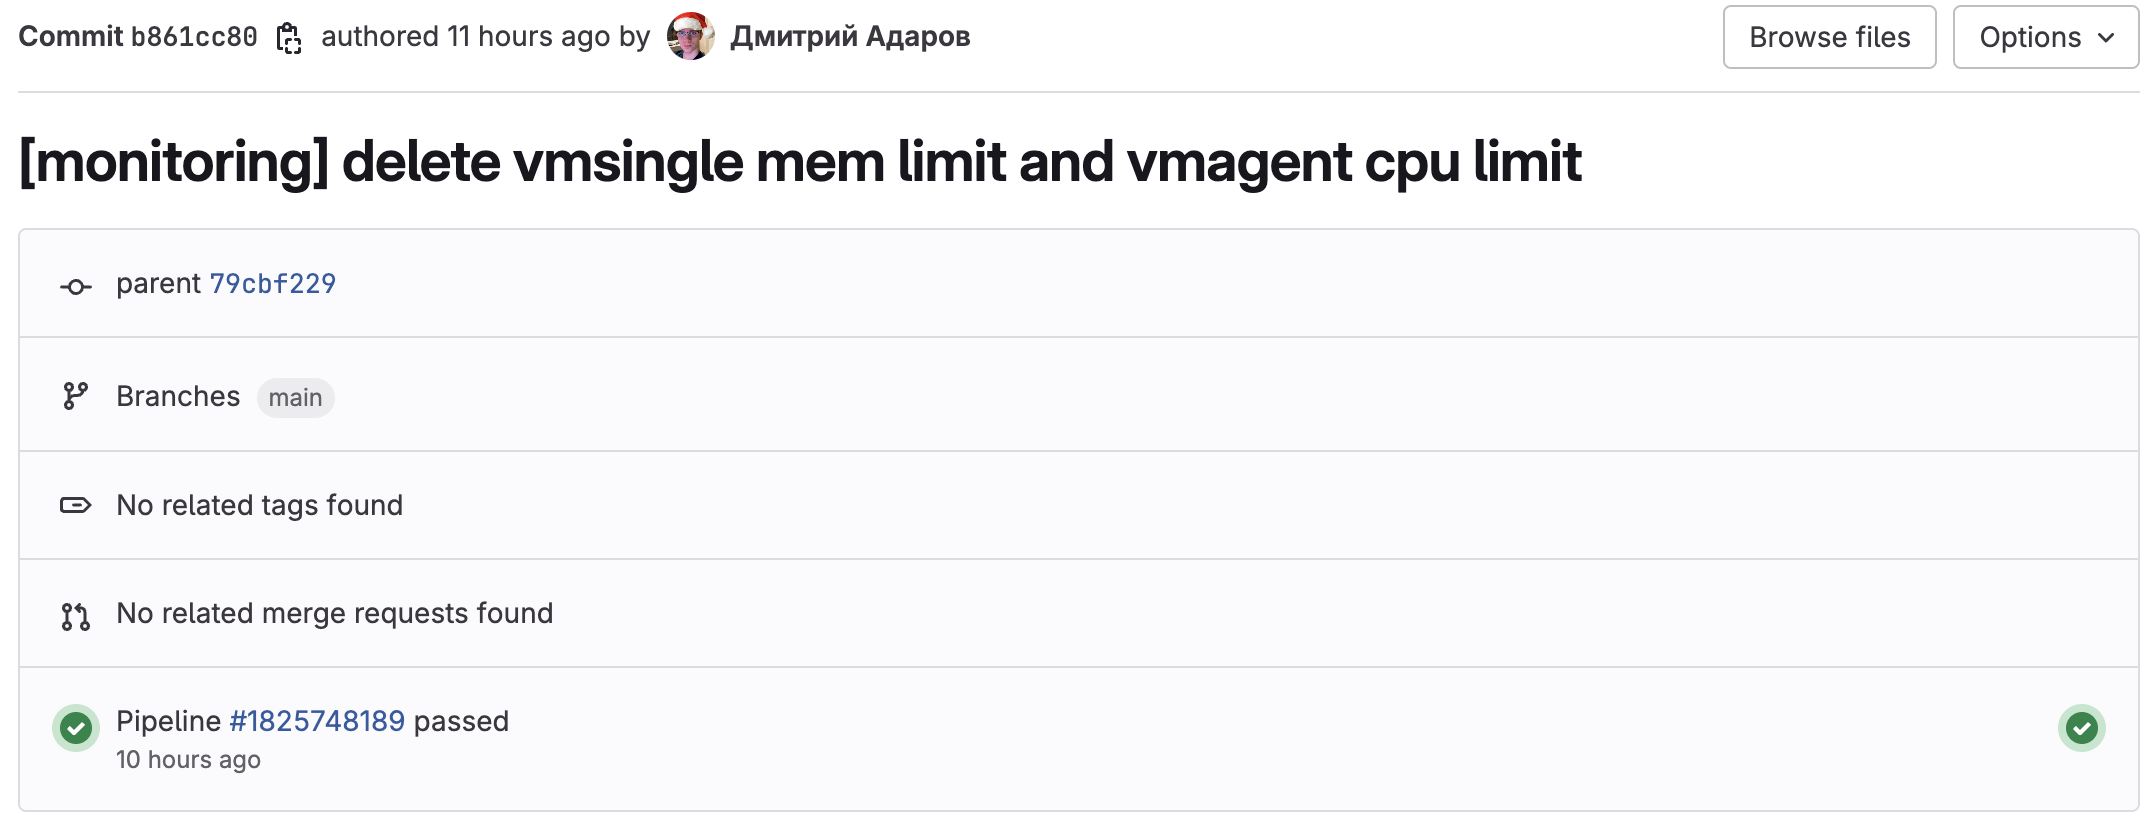
\includegraphics[width=0.7\linewidth]{\commonSecPathPrefix/../img/sec_6/ci_pipeline.png}
    \caption{Общий вид пайплайна в интерфейсе \textit{GitLab}}
    \label{fig:user_guide:ci_pipeline}
\end{figure}

На рисунке \ref{fig:user_guide:ci_pipeline} можно выделить следующие элементы:
\begin{itemize}
    \item стадии пайплайна, например: \textit{lint}, \textit{test}, \textit{deploy};
    \item статус выполнения задач: \textit{passed}, \textit{failed}, \textit{skipped}, \textit{manual};
    \item возможность запуска ручных этапов с помощью флага \textit{when: manual};
    \item переход к логам выполнения каждой задачи для детальной диагностики;
    \item визуальные индикаторы статуса с цветовой кодировкой (зелёный, красный, серый).
\end{itemize}

Запуск и управление \textit{Ansible}-плейбуками также интегрированы в \textit{GitLab CI}. Это позволяет упростить процесс настройки и сопровождения инфраструктуры. На рисунке \ref{fig:user_guide:ci_ansible} показан один из таких шагов.

\begin{figure}[ht]
    \centering
    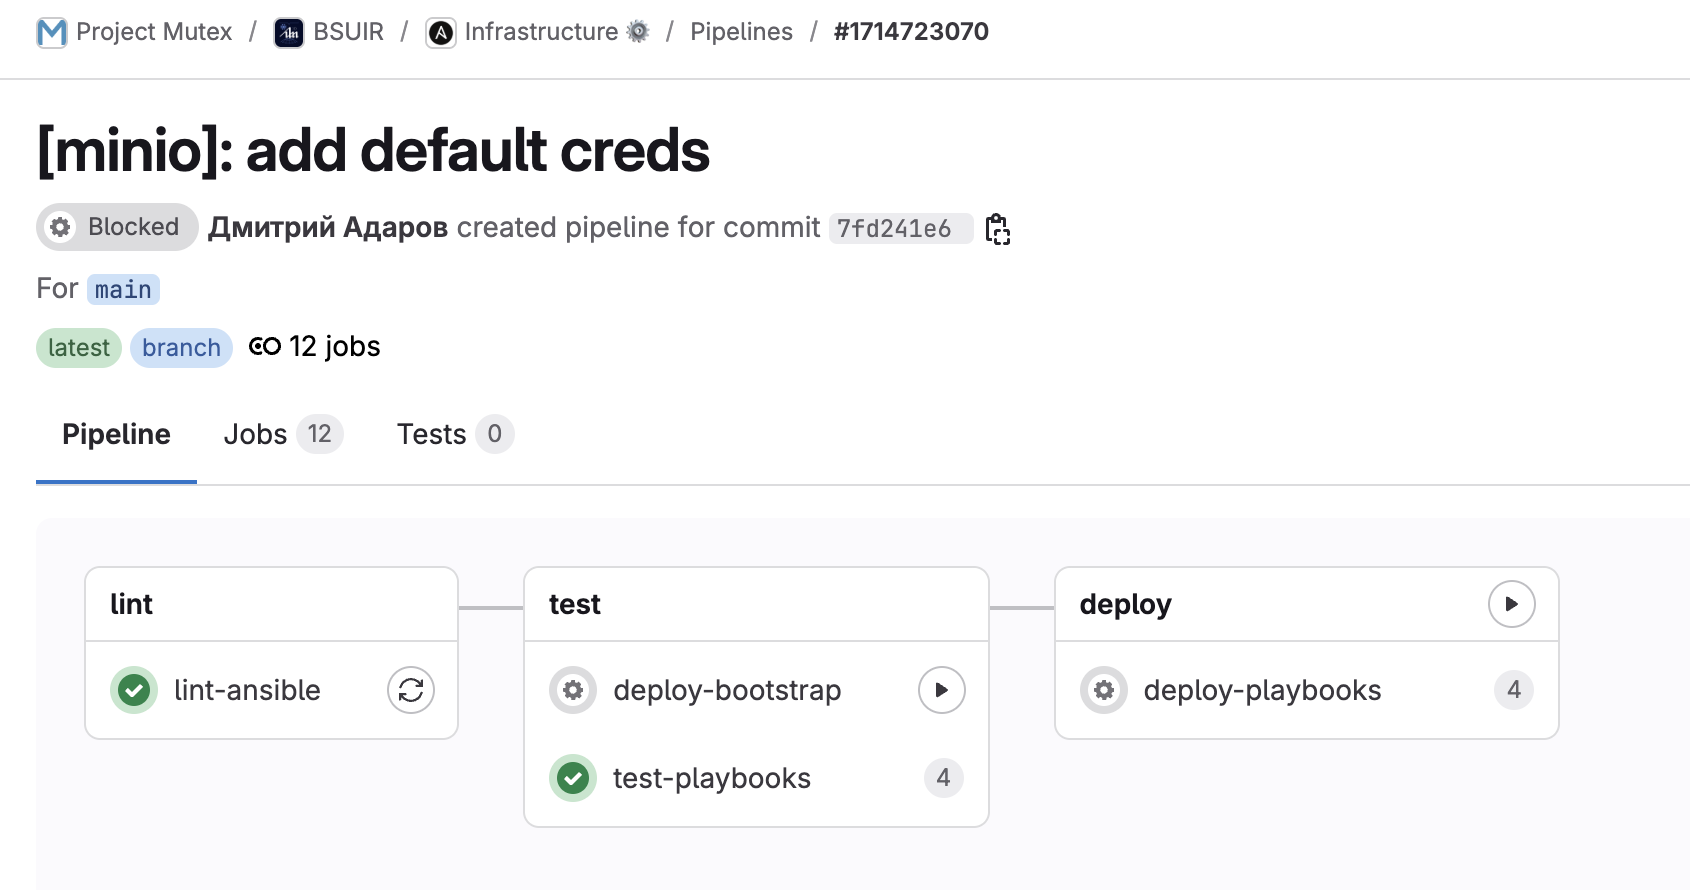
\includegraphics[width=0.7\linewidth]{\commonSecPathPrefix/../img/sec_6/ci_ansible.png}
    \caption{Интерфейс запуска \textit{Ansible}-плейбуков из \textit{GitLab CI}}
    \label{fig:user_guide:ci_ansible}
\end{figure}

Пользователю предоставляется возможность:
\begin{itemize}
    \item выбрать необходимый плейбук из набора доступных, например, \textit{k3s.yaml};
    \item указать параметры командной строки для точной настройки задачи;
    \item отслеживать выполнение команд \lstinline{ansible-playbook} в реальном времени;
    \item идентифицировать инициатора запуска и дату выполнения;
    \item быстро получить доступ к логам, чтобы проанализировать результаты или устранить ошибки.
\end{itemize}

\subsection{Система управления доступом (\textit{IDM})}

Система идентификации и управления доступом реализована на базе \textit{Authentik}. Она обеспечивает единую точку входа для всех сервисов, централизованное управление пользователями, поддерживает различные протоколы авторизации (\textit{OAuth2}, \textit{LDAP}, \textit{SAML}) и предоставляет гибкие возможности для настройки политик безопасности.

\begin{figure}[ht]
    \centering
    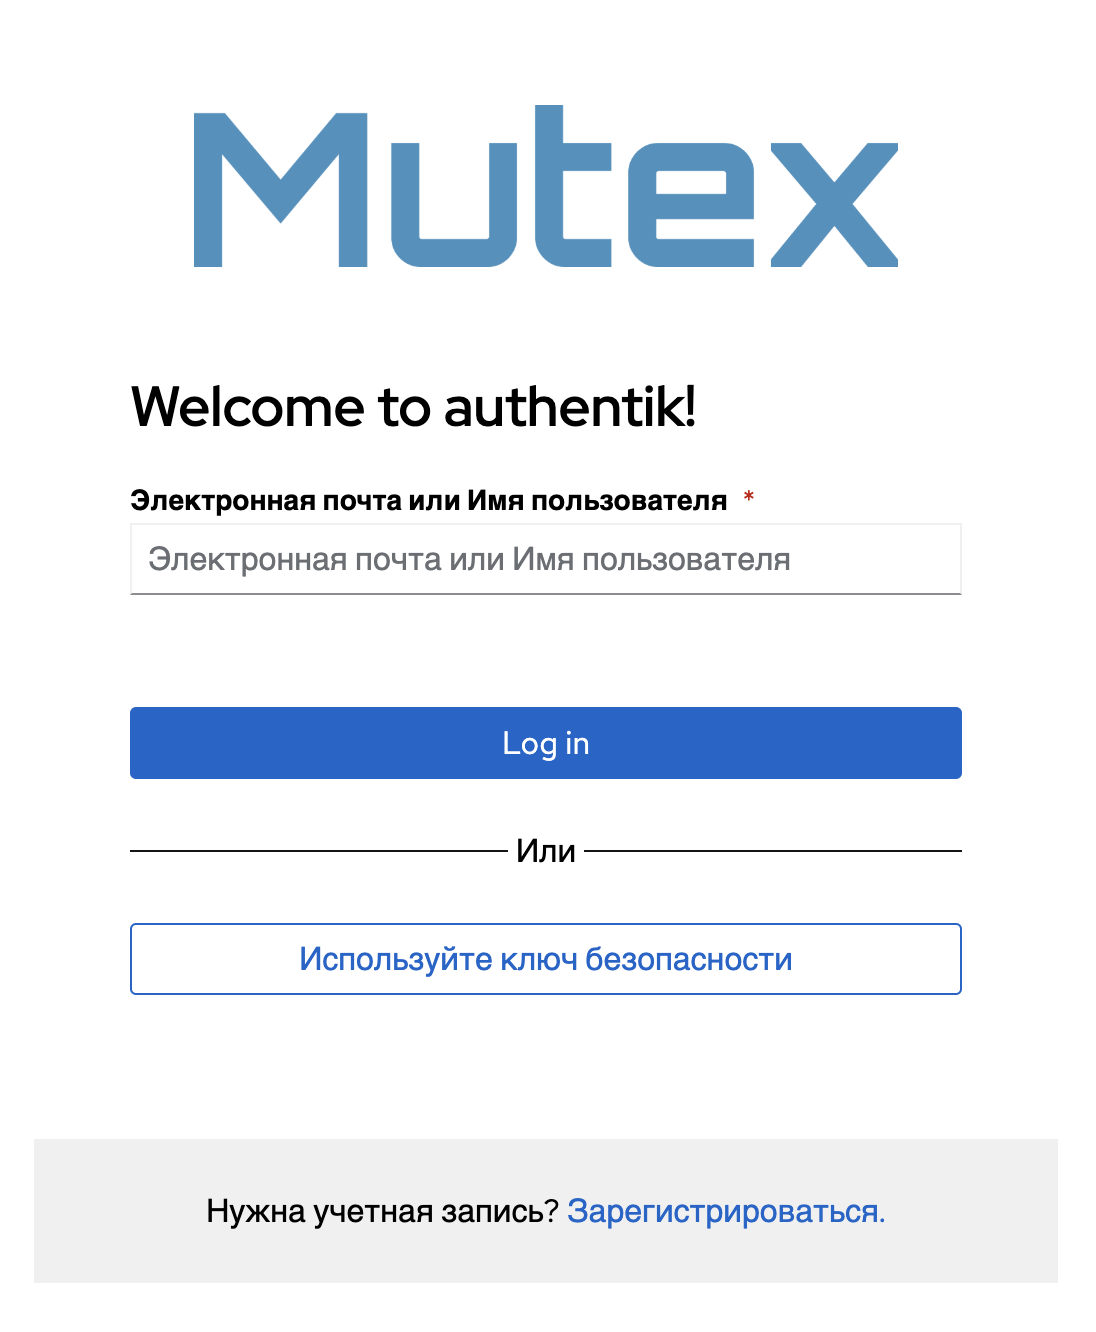
\includegraphics[width=0.5\linewidth]{\commonSecPathPrefix/../img/sec_6/idm_login.png}
    \caption{Страница входа в \textit{Authentik}}
    \label{fig:user_guide:idm_login}
\end{figure}

На рисунке \ref{fig:user_guide:idm_login} представлена форма аутентификации:
\begin{itemize}
    \item поле для ввода имени пользователя или электронной почты;
    \item поле для ввода пароля;
    \item кнопка входа через сторонние сервисы, например, \textit{GitHub}, \textit{Google};
    \item возможность восстановления доступа с помощью ссылки \textit{Forgot password?}.
\end{itemize}

После входа пользователь попадает на домашнюю страницу (\ref{fig:user_guide:idm_home}), где отображаются доступные ему ресурсы и информация об активной сессии.

\begin{figure}[ht]
    \centering
    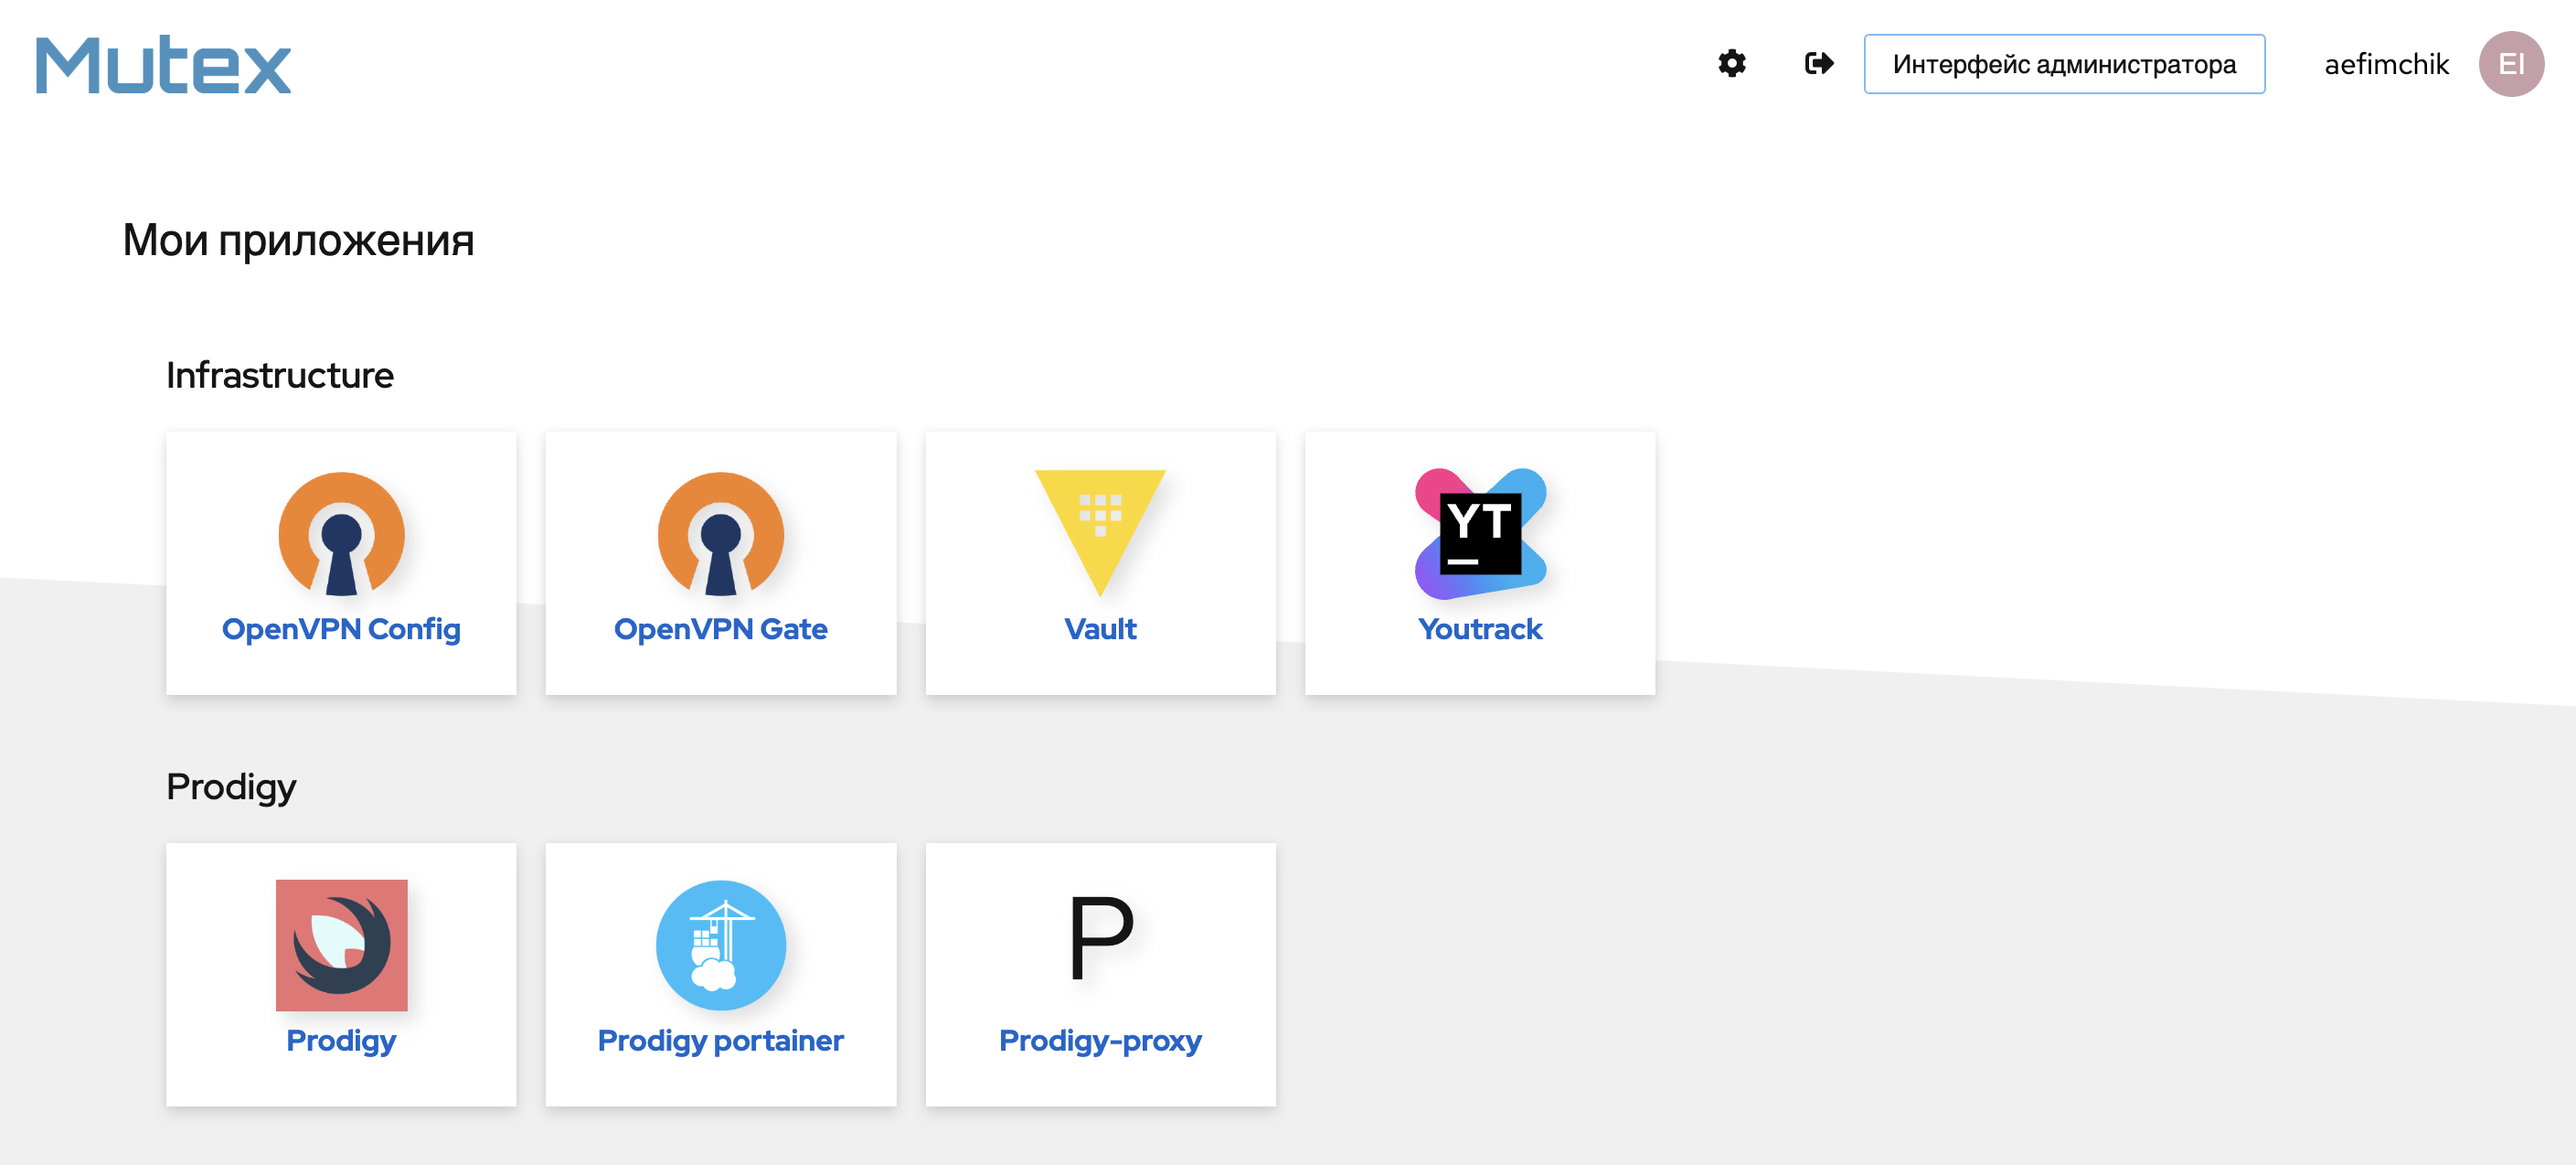
\includegraphics[width=0.7\linewidth]{\commonSecPathPrefix/../img/sec_6/idm_home.png}
    \caption{Домашняя страница пользователя в \textit{Authentik}}
    \label{fig:user_guide:idm_home}
\end{figure}

В интерфейсе доступны:
\begin{itemize}
    \item список приложений, к которым у пользователя есть доступ;
    \item сведения об активных сессиях, \textit{IP}-адресах, времени последней активности;
    \item возможность выхода из системы и сброса пароля;
    \item профиль пользователя с контактными данными и группами.
\end{itemize}

Для администраторов предусмотрен отдельный интерфейс, представленный на рисунке \ref{fig:user_guide:idm_admin}.

\begin{figure}[ht]
    \centering
    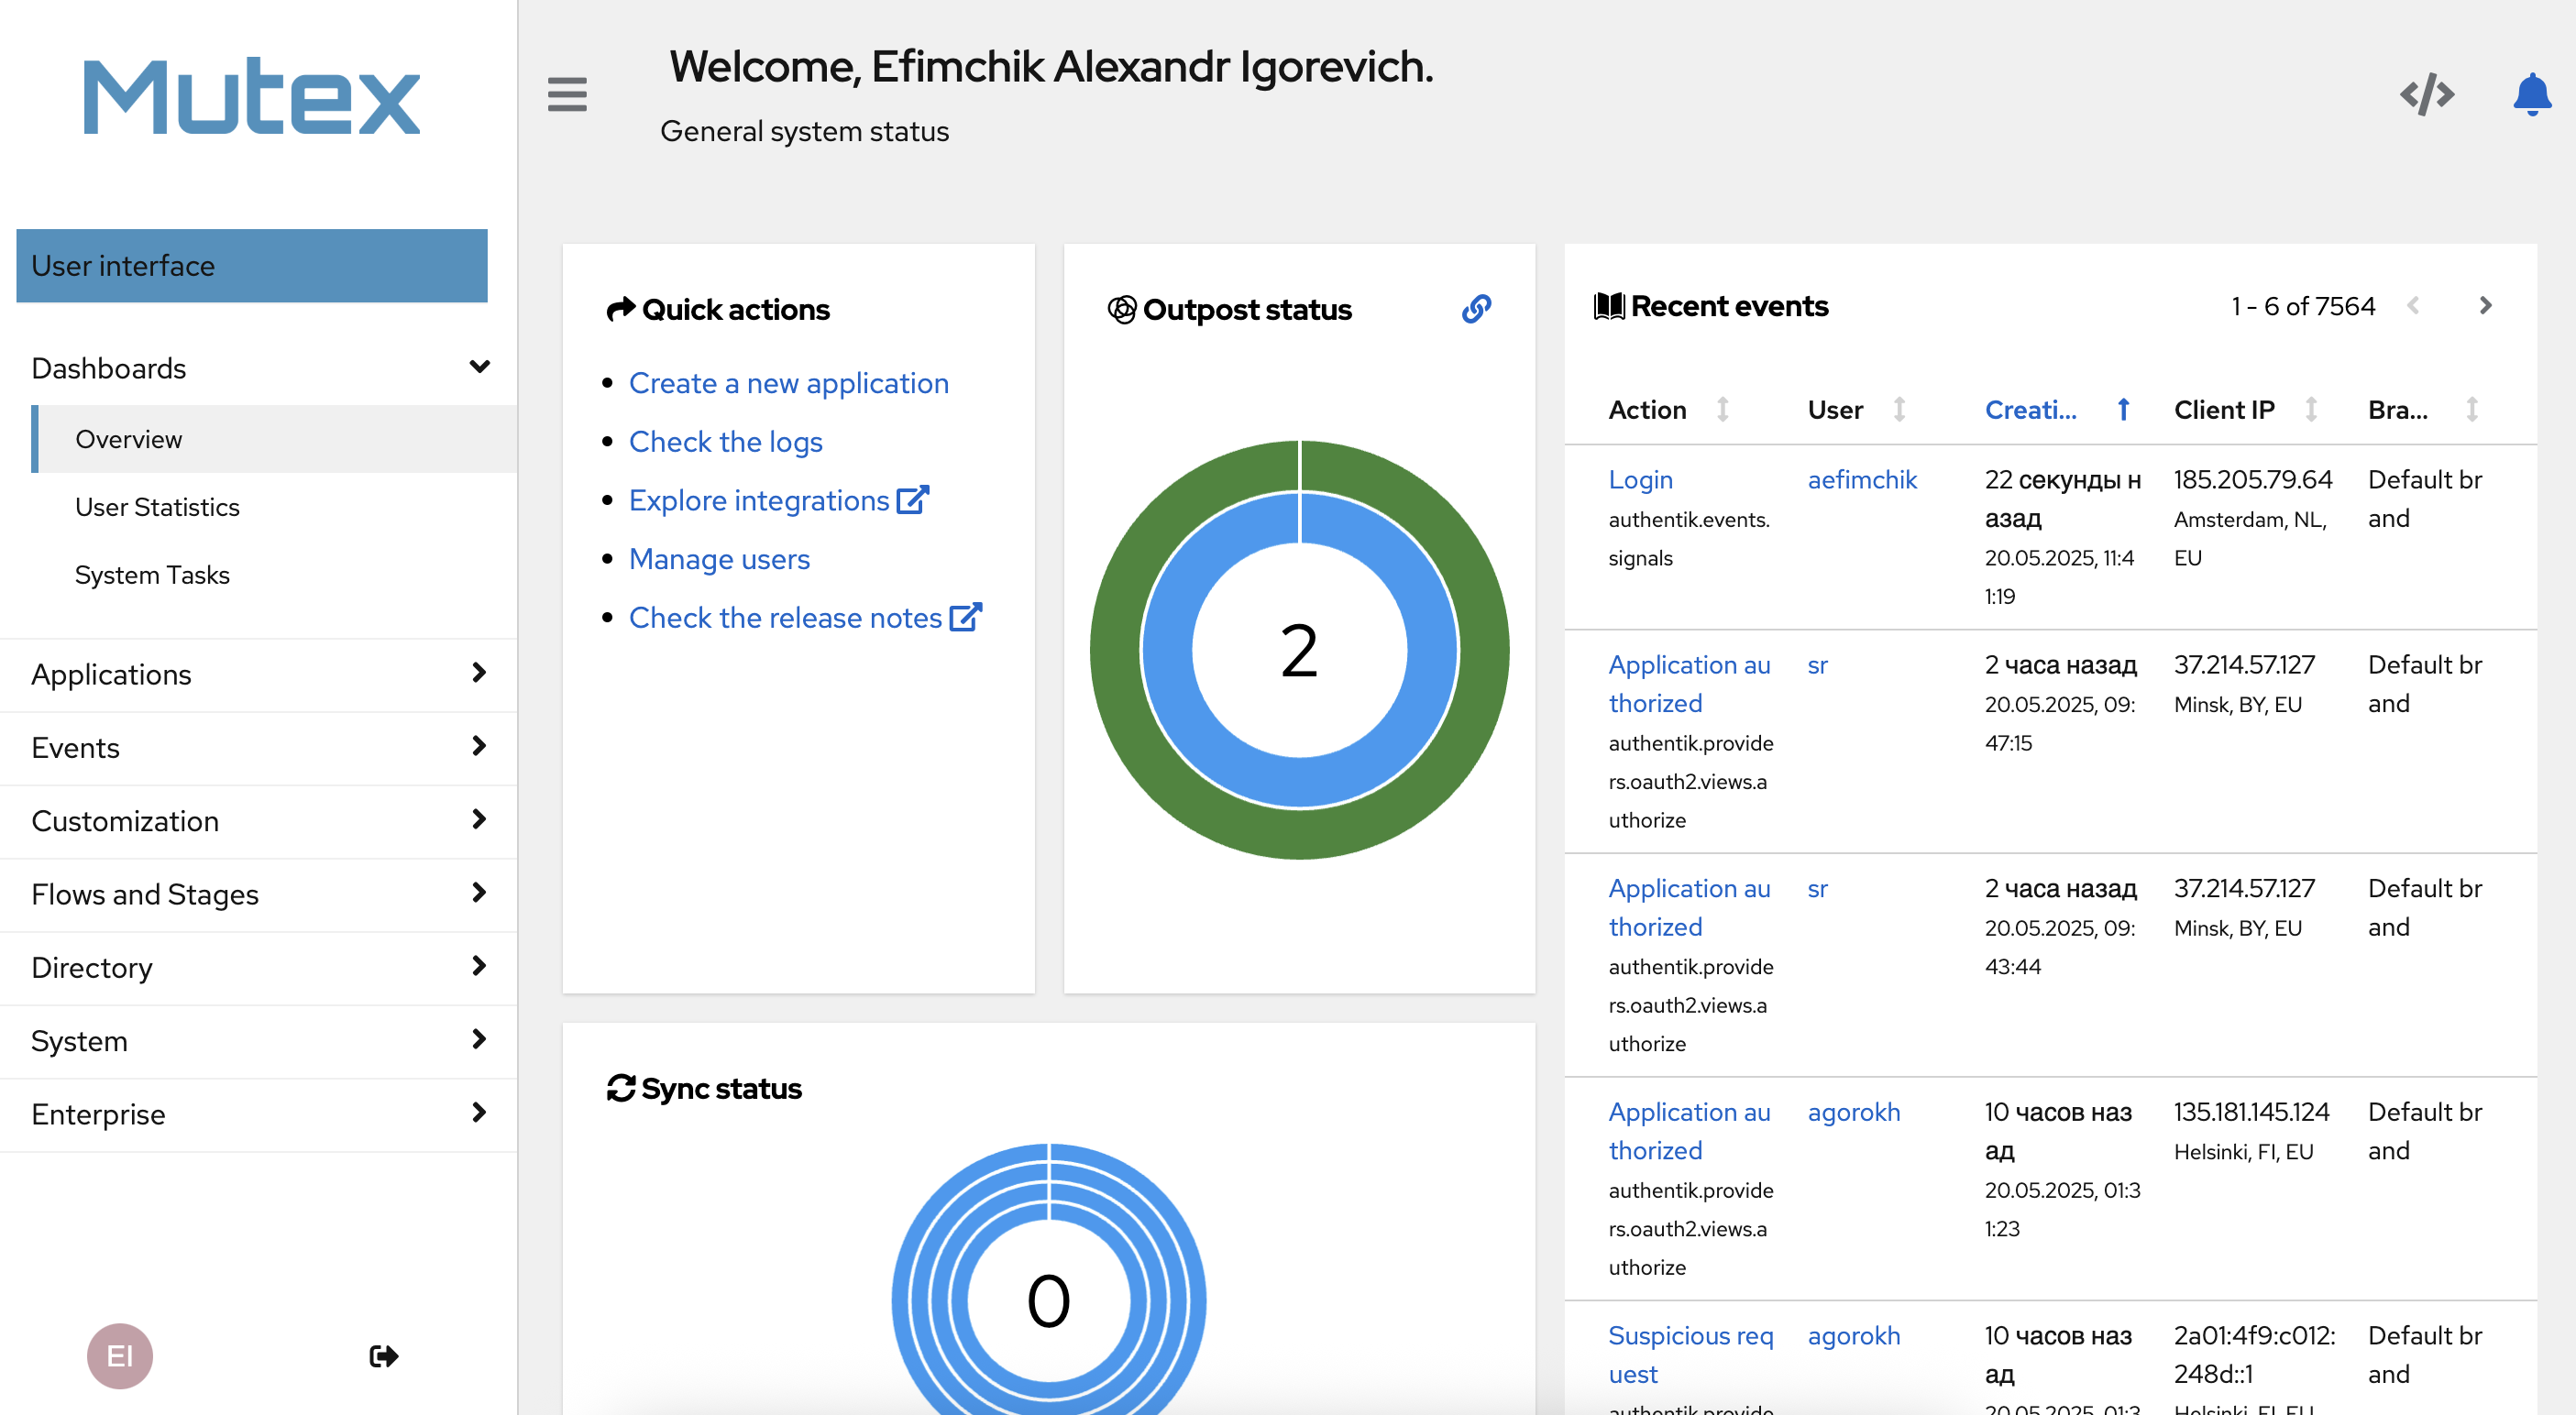
\includegraphics[width=0.7\linewidth]{\commonSecPathPrefix/../img/sec_6/idm_admin.png}
    \caption{Панель администратора \textit{Authentik}}
    \label{fig:user_guide:idm_admin}
\end{figure}

В административной панели доступны:
\begin{itemize}
    \item управление пользователями, группами, токенами и сессиями;
    \item настройка политик доступа с использованием условных правил;
    \item подключение внешних провайдеров авторизации;
    \item просмотр логов входов, попыток аутентификации и действий пользователей.
\end{itemize}

Управление группами, правами и назначением ролей реализовано в соответствующем разделе (рисунок \ref{fig:user_guide:idm_group}).

\begin{figure}[ht]
    \centering
    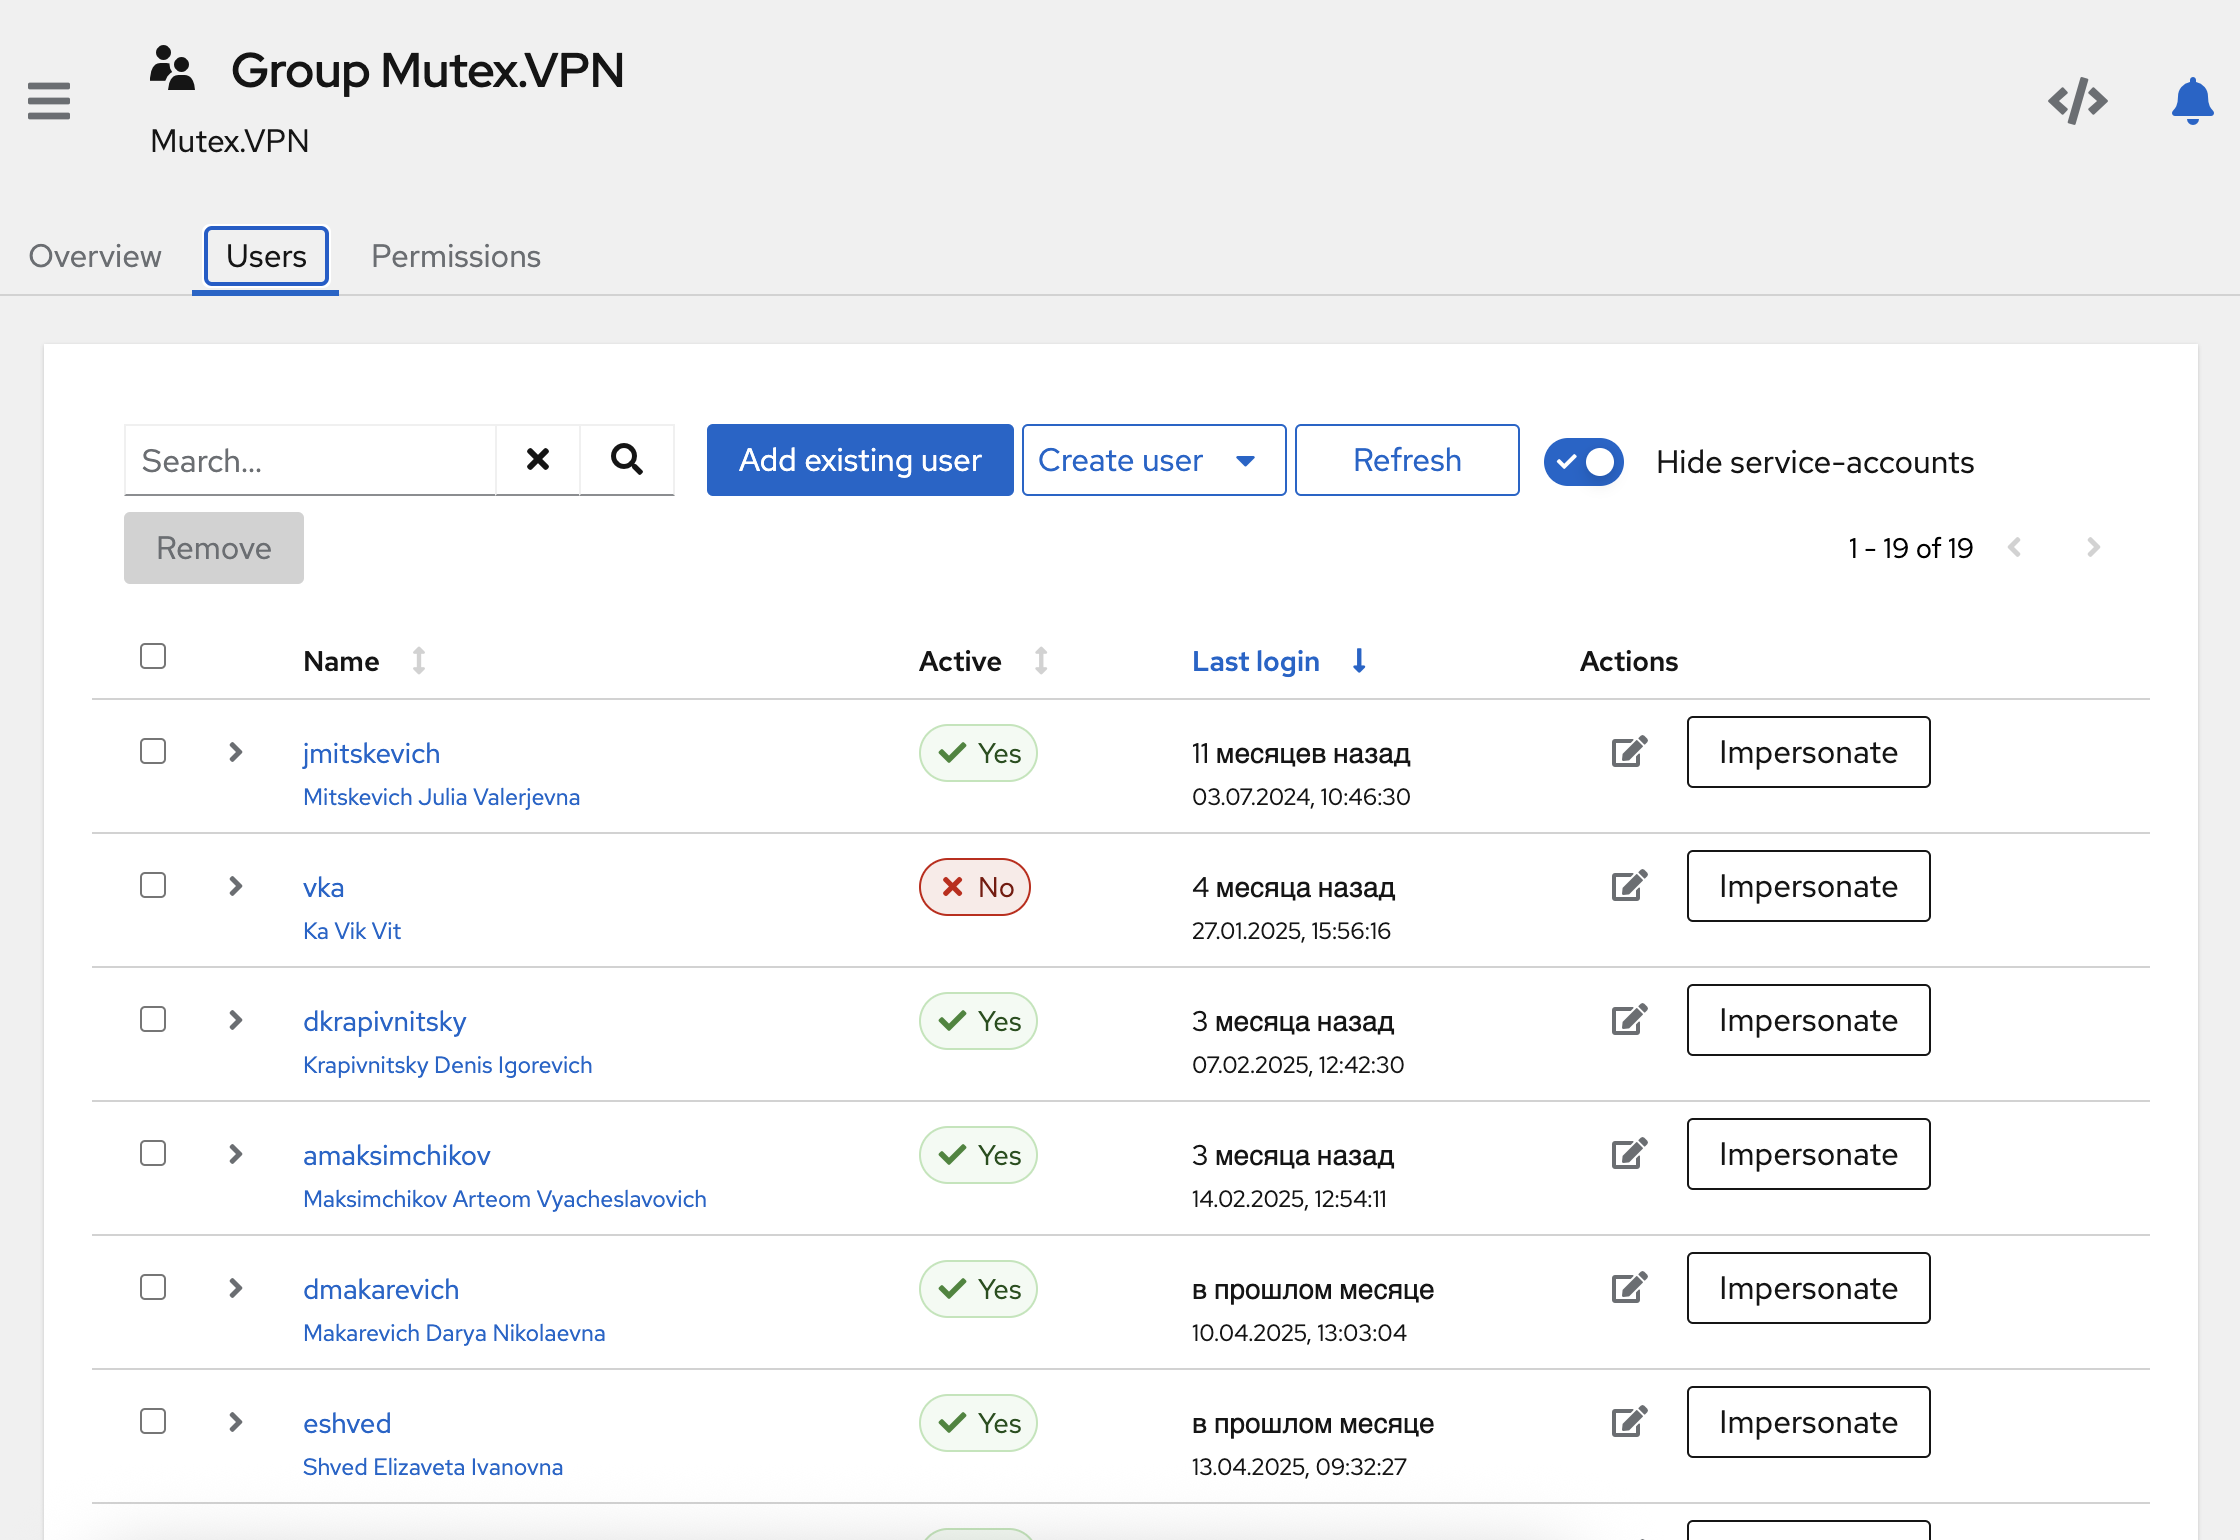
\includegraphics[width=0.7\linewidth]{\commonSecPathPrefix/../img/sec_6/idm_group.png}
    \caption{Управление группами пользователей в \textit{Authentik}}
    \label{fig:user_guide:idm_group}
\end{figure}

В панели администратора возможно:
\begin{itemize}
    \item создавать и удалять группы;
    \item добавлять и исключать пользователей;
    \item задавать роли и уровни доступа;
    \item применять политики к приложениям, \textit{API} или внутренним ресурсам.
\end{itemize}

\subsection{Интерфейс мониторинга (\textit{Grafana})}

Для сбора и анализа метрик используется связка \textit{VictoriaMetrics} и \textit{Grafana}, которая предоставляет мощный графический интерфейс. Пользователи могут наблюдать за состоянием компонентов системы, проводить анализ отклонений, строить собственные графики на языке \textit{PromQL}.

\begin{figure}[ht]
    \centering
    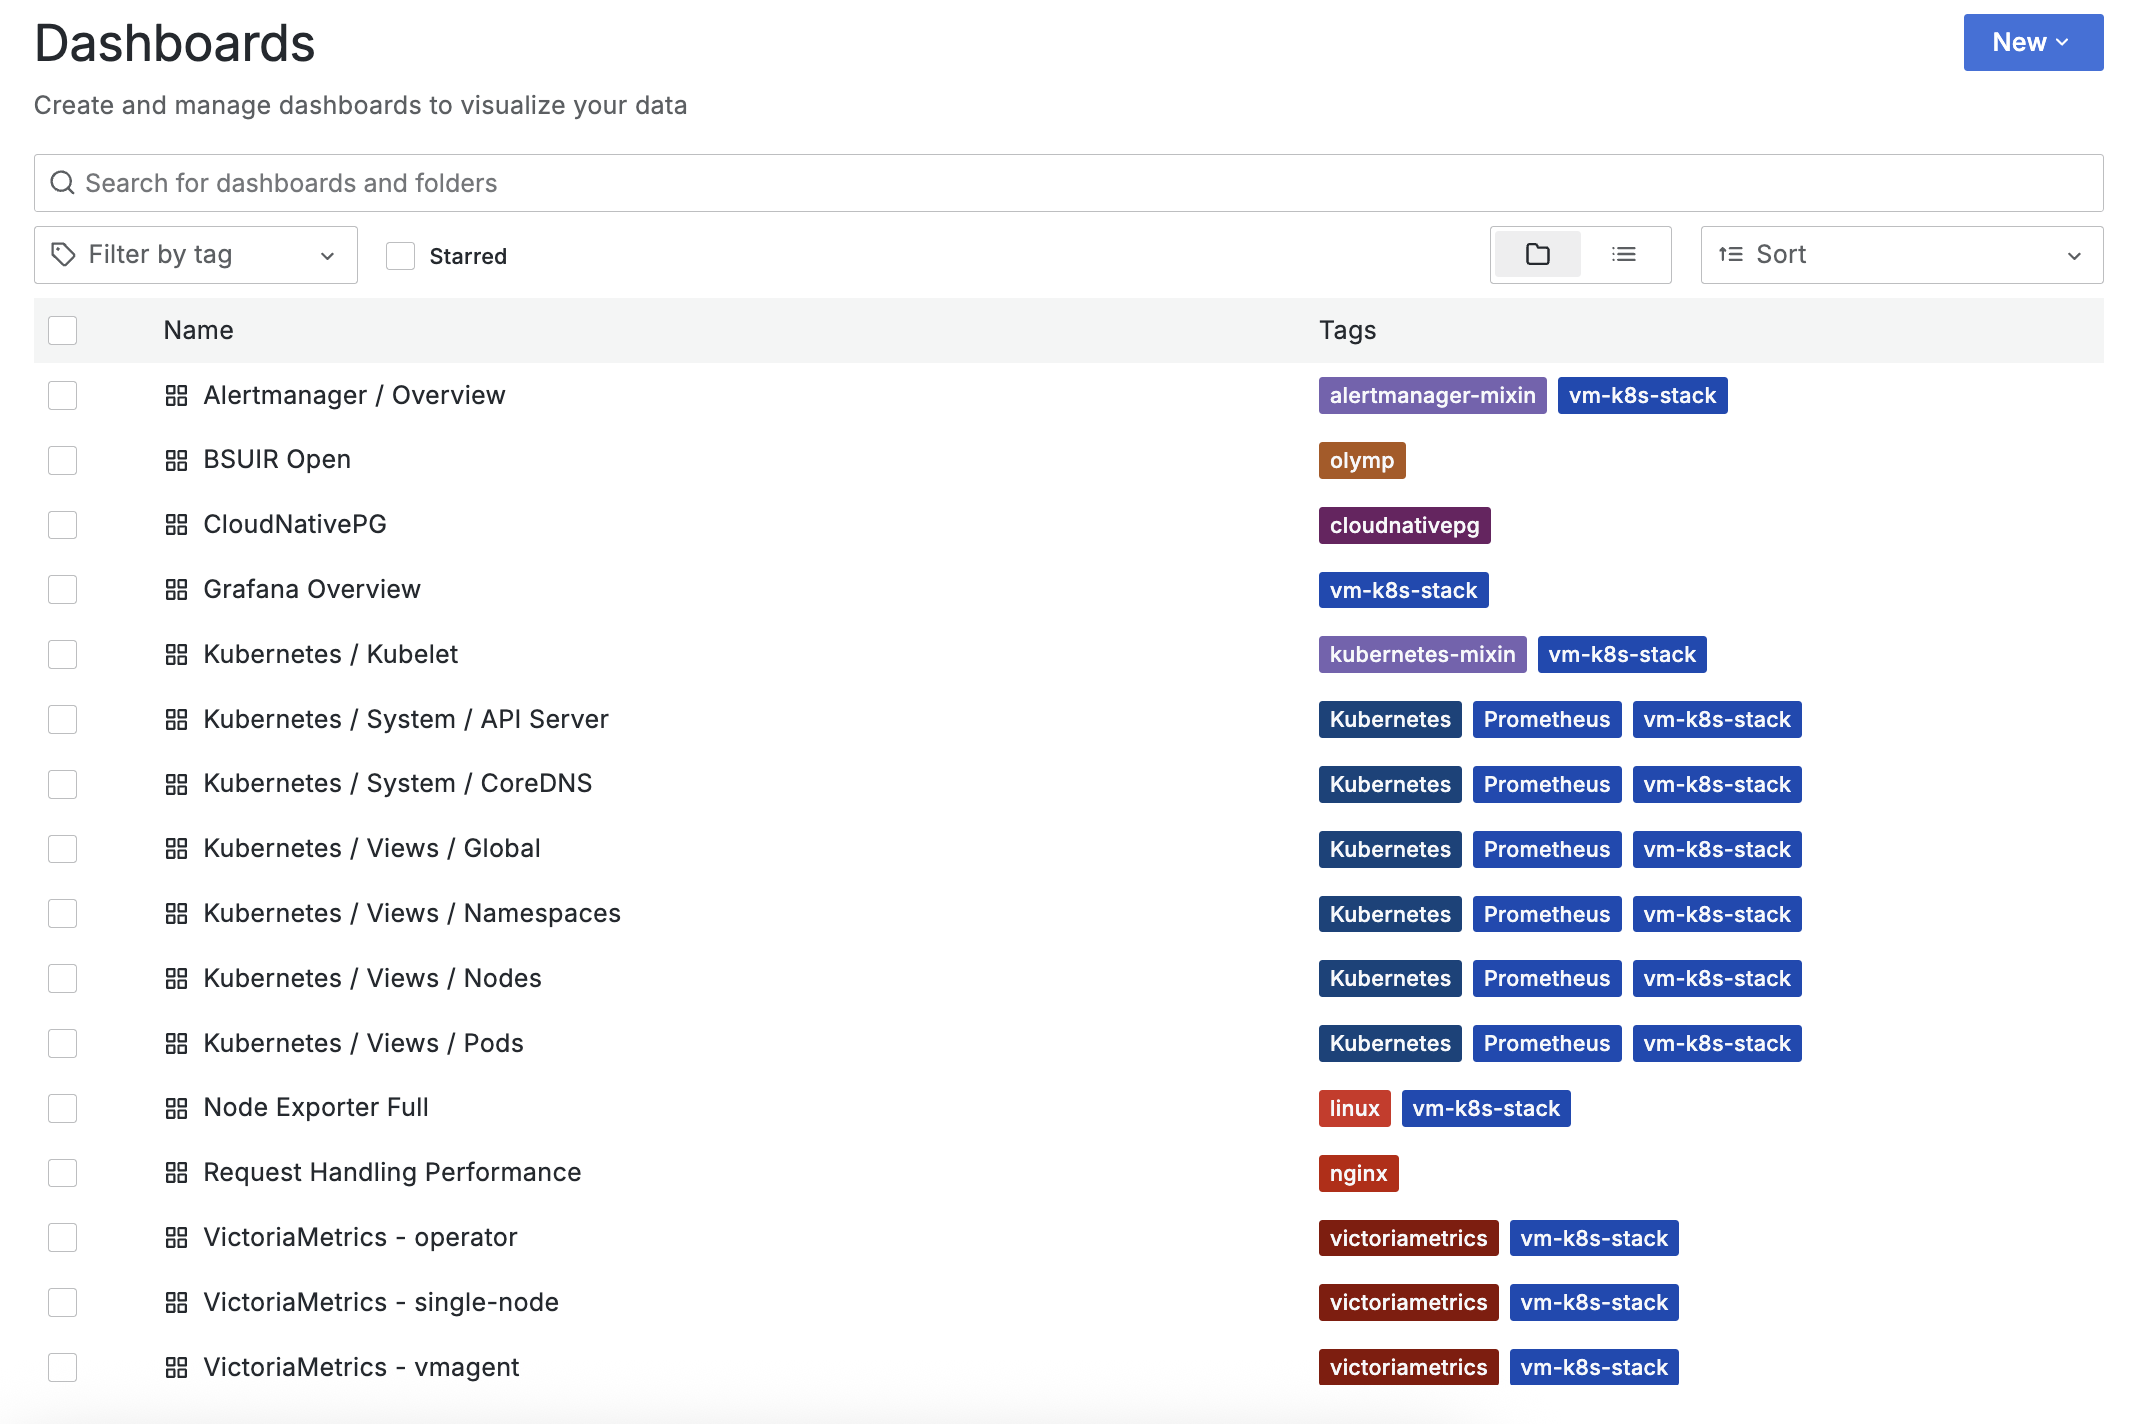
\includegraphics[width=0.7\linewidth]{\commonSecPathPrefix/../img/sec_6/grafana_dashboards.png}
    \caption{Список доступных дашбордов в \textit{Grafana}}
    \label{fig:user_guide:grafana_dashboards}
\end{figure}

Интерфейс позволяет:
\begin{itemize}
    \item осуществлять поиск по названию дашборда;
    \item закреплять избранные панели;
    \item фильтровать по папкам, тегам, источникам данных;
    \item просматривать метаданные дашборда: описание, автор, дата последнего изменения.
\end{itemize}

\textit{Grafana} поддерживает гибкую организацию дашбордов, что позволяет удобно структурировать информацию по функциональным областям или группам сервисов. Это облегчает работу специалистов, отвечающих за мониторинг, и ускоряет выявление проблемных участков.

Настраиваемые права доступа позволяют ограничивать просмотр или редактирование конкретных дашбордов для различных групп пользователей, что обеспечивает безопасность и соответствие корпоративным политикам.

Визуализация данных может включать не только стандартные графики, но и диаграммы, таблицы, тепловые карты и другие виды представлений. Это даёт возможность глубоко анализировать метрики и быстро принимать решения по инцидентам.

Открыв конкретный дашборд, пользователь получает доступ к визуализации ключевых метрик. Пример такой визуализации представлен на рисунке \ref{fig:user_guide:grafana_dashboard}.

\begin{figure}[ht]
    \centering
    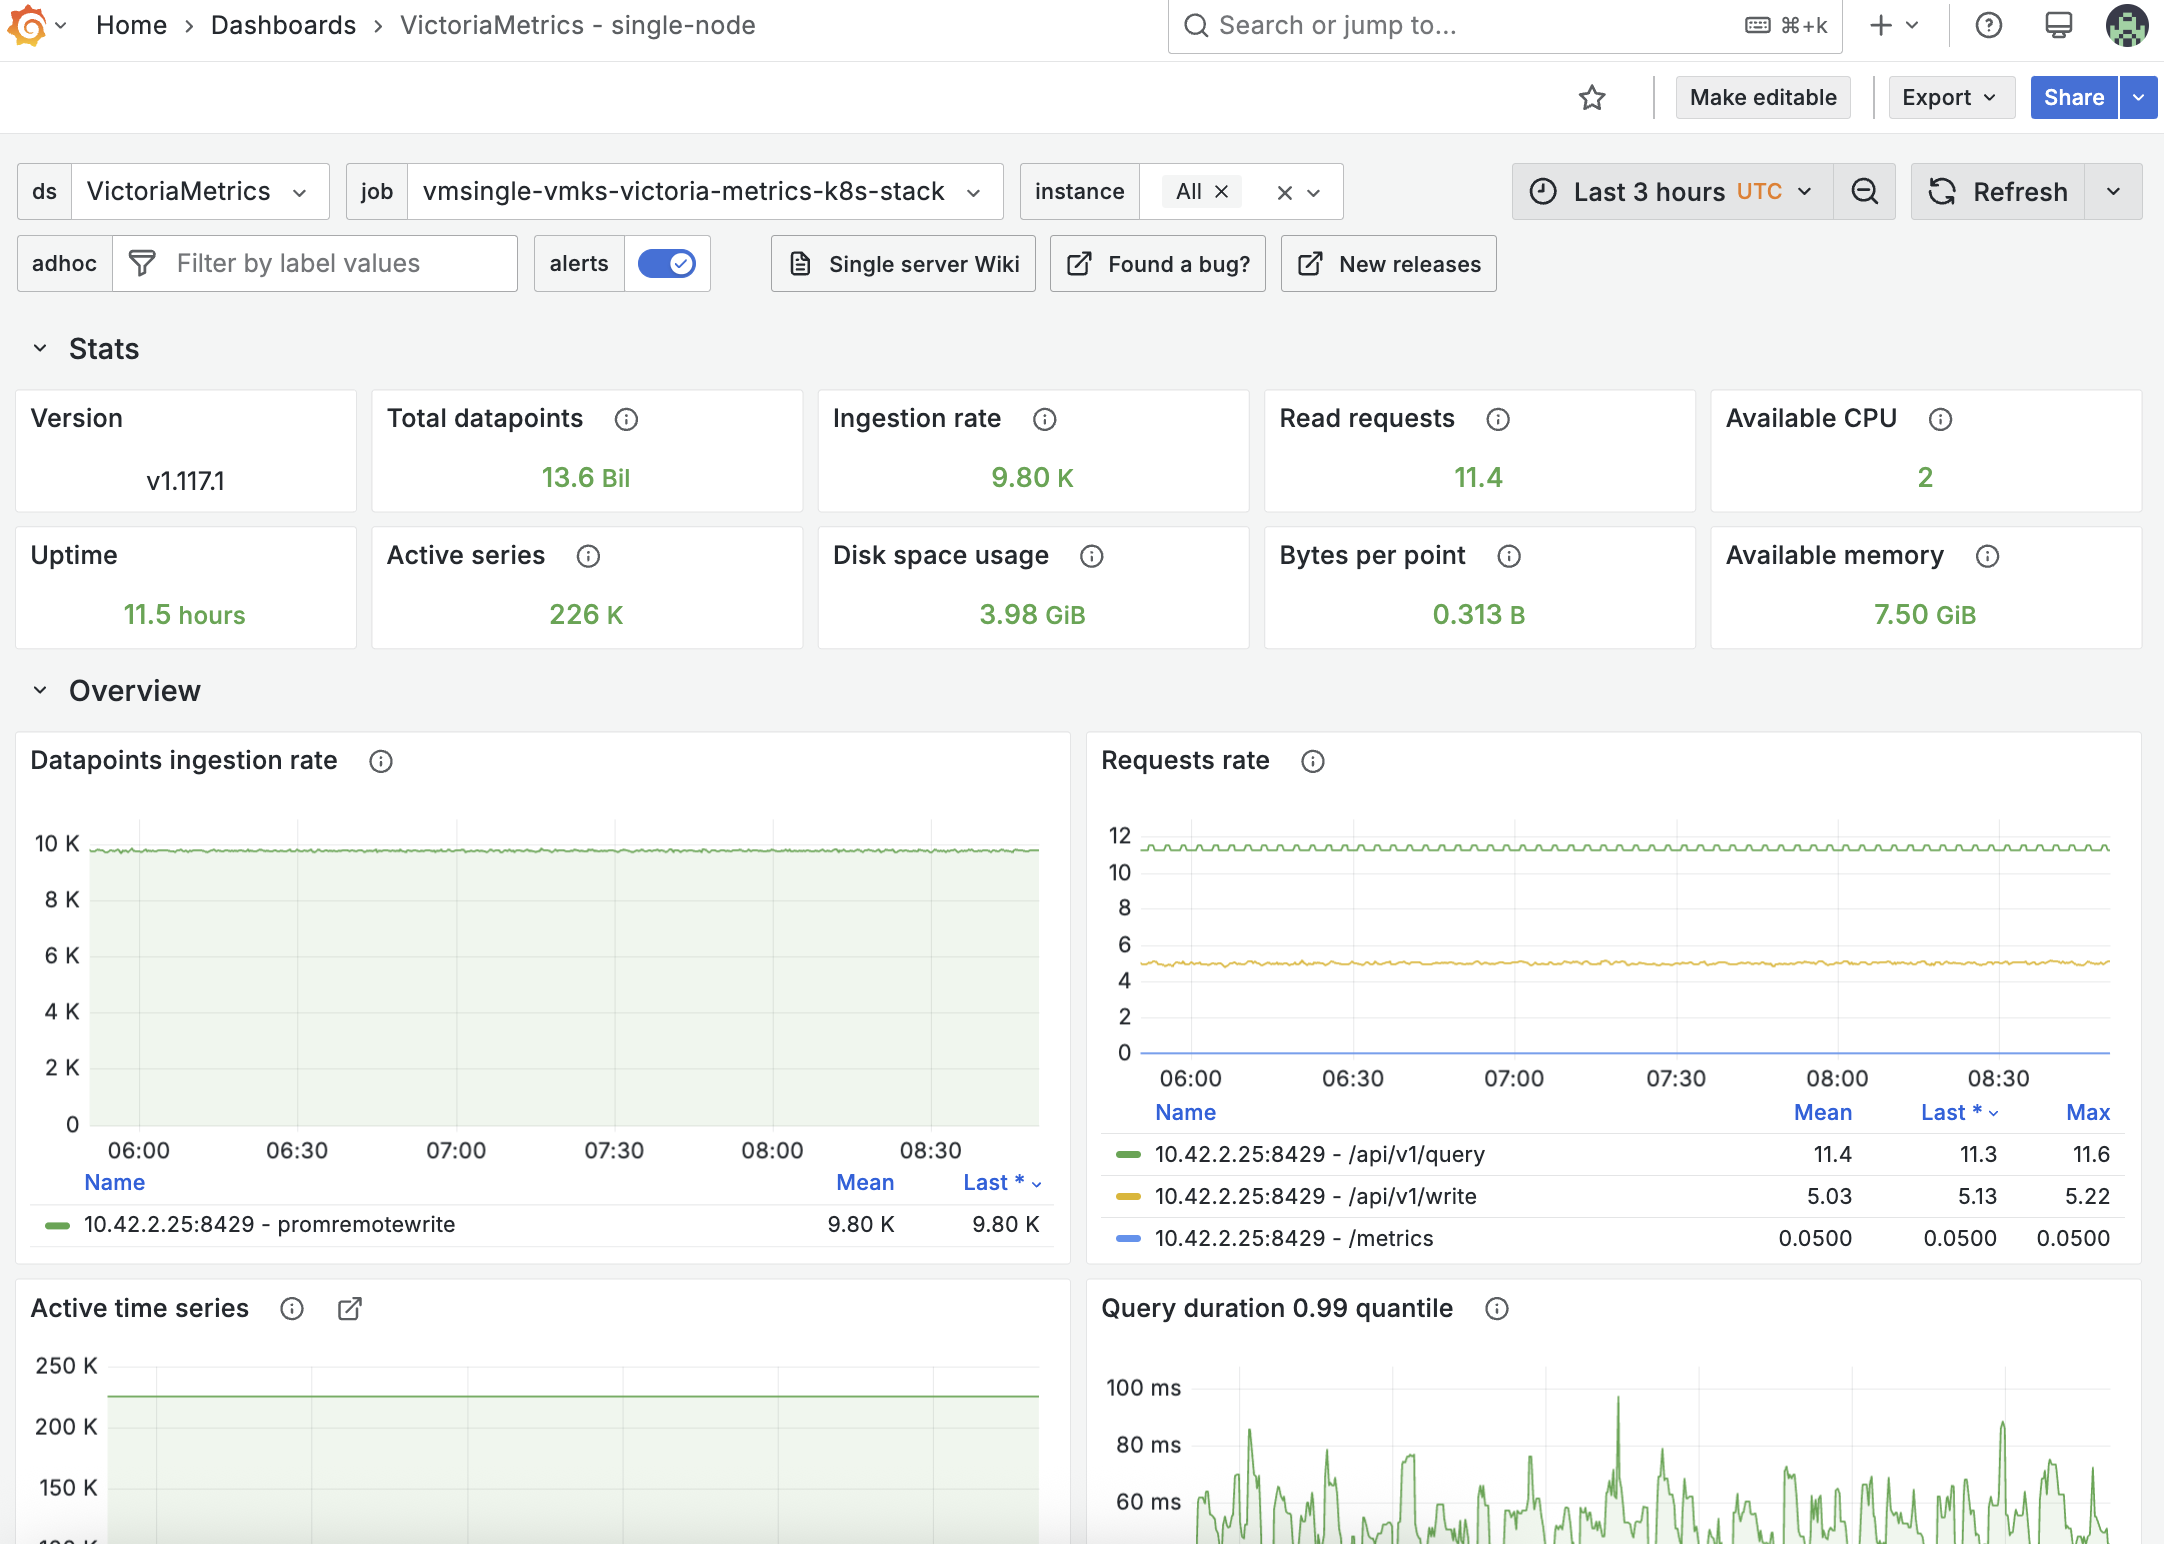
\includegraphics[width=0.67\linewidth]{\commonSecPathPrefix/../img/sec_6/grafana_dashboard.png}
    \caption{Пример дашборда мониторинга в \textit{Grafana}}
    \label{fig:user_guide:grafana_dashboard}
\end{figure}

Панели содержат:
\begin{itemize}
    \item графики загрузки \textit{CPU}, использования \textit{RAM}, сетевого трафика;
    \item шкалы времени, легенды, фильтры по подмножествам данных;
    \item возможность редактировать запросы и строить пользовательские панели;
    \item экспорт графиков в изображение или \textit{PDF}, а также шаринг по ссылке.
\end{itemize}

Кроме стандартных возможностей, \textit{Grafana} поддерживает уведомления и интеграции с внешними системами оповещений, такими как \textit{Slack}, \textit{Email} или \textit{PagerDuty}. Это позволяет оперативно информировать ответственных сотрудников о критических изменениях состояния инфраструктуры.

Интерфейс \textit{Grafana} адаптивен и может использоваться как на десктопах, так и на мобильных устройствах, обеспечивая круглосуточный доступ к мониторингу и повышая эффективность управления системой.

Визуальные панели \textit{Grafana} позволяют быстро оценивать тенденции и аномалии, что способствует более проактивному подходу в эксплуатации инфраструктуры.

Кроме того, система поддерживает расширения и плагины, которые позволяют интегрировать сторонние источники данных и адаптировать интерфейс под специфические задачи компании.

Таким образом, применение \textit{Grafana} в рамках отказоустойчивой инфраструктуры компании позволяет не только контролировать состояние ресурсов в режиме реального времени, но и строить прогнозы на основе исторических данных для предотвращения инцидентов.


\subsection{Интерфейс управления секретами (\textit{HashiCorp Vault})}

\textit{HashiCorp Vault} -- это мощное средство для централизованного управления секретами и конфиденциальными данными, такими как токены доступа, пароли, ключи шифрования и сертификаты. Основная задача \textit{Vault} —- обеспечить безопасное хранение, контролируемый доступ и аудит всех операций с секретами в корпоративной инфраструктуре.

В проекте \textit{Vault} интегрирован в \textit{IT}-инфраструктуру для решения задач управления доступом к чувствительным данным, автоматизации выпуска сертификатов и обеспечения сквозного контроля версий и политики безопасности.

\begin{figure}[ht]
    \centering
    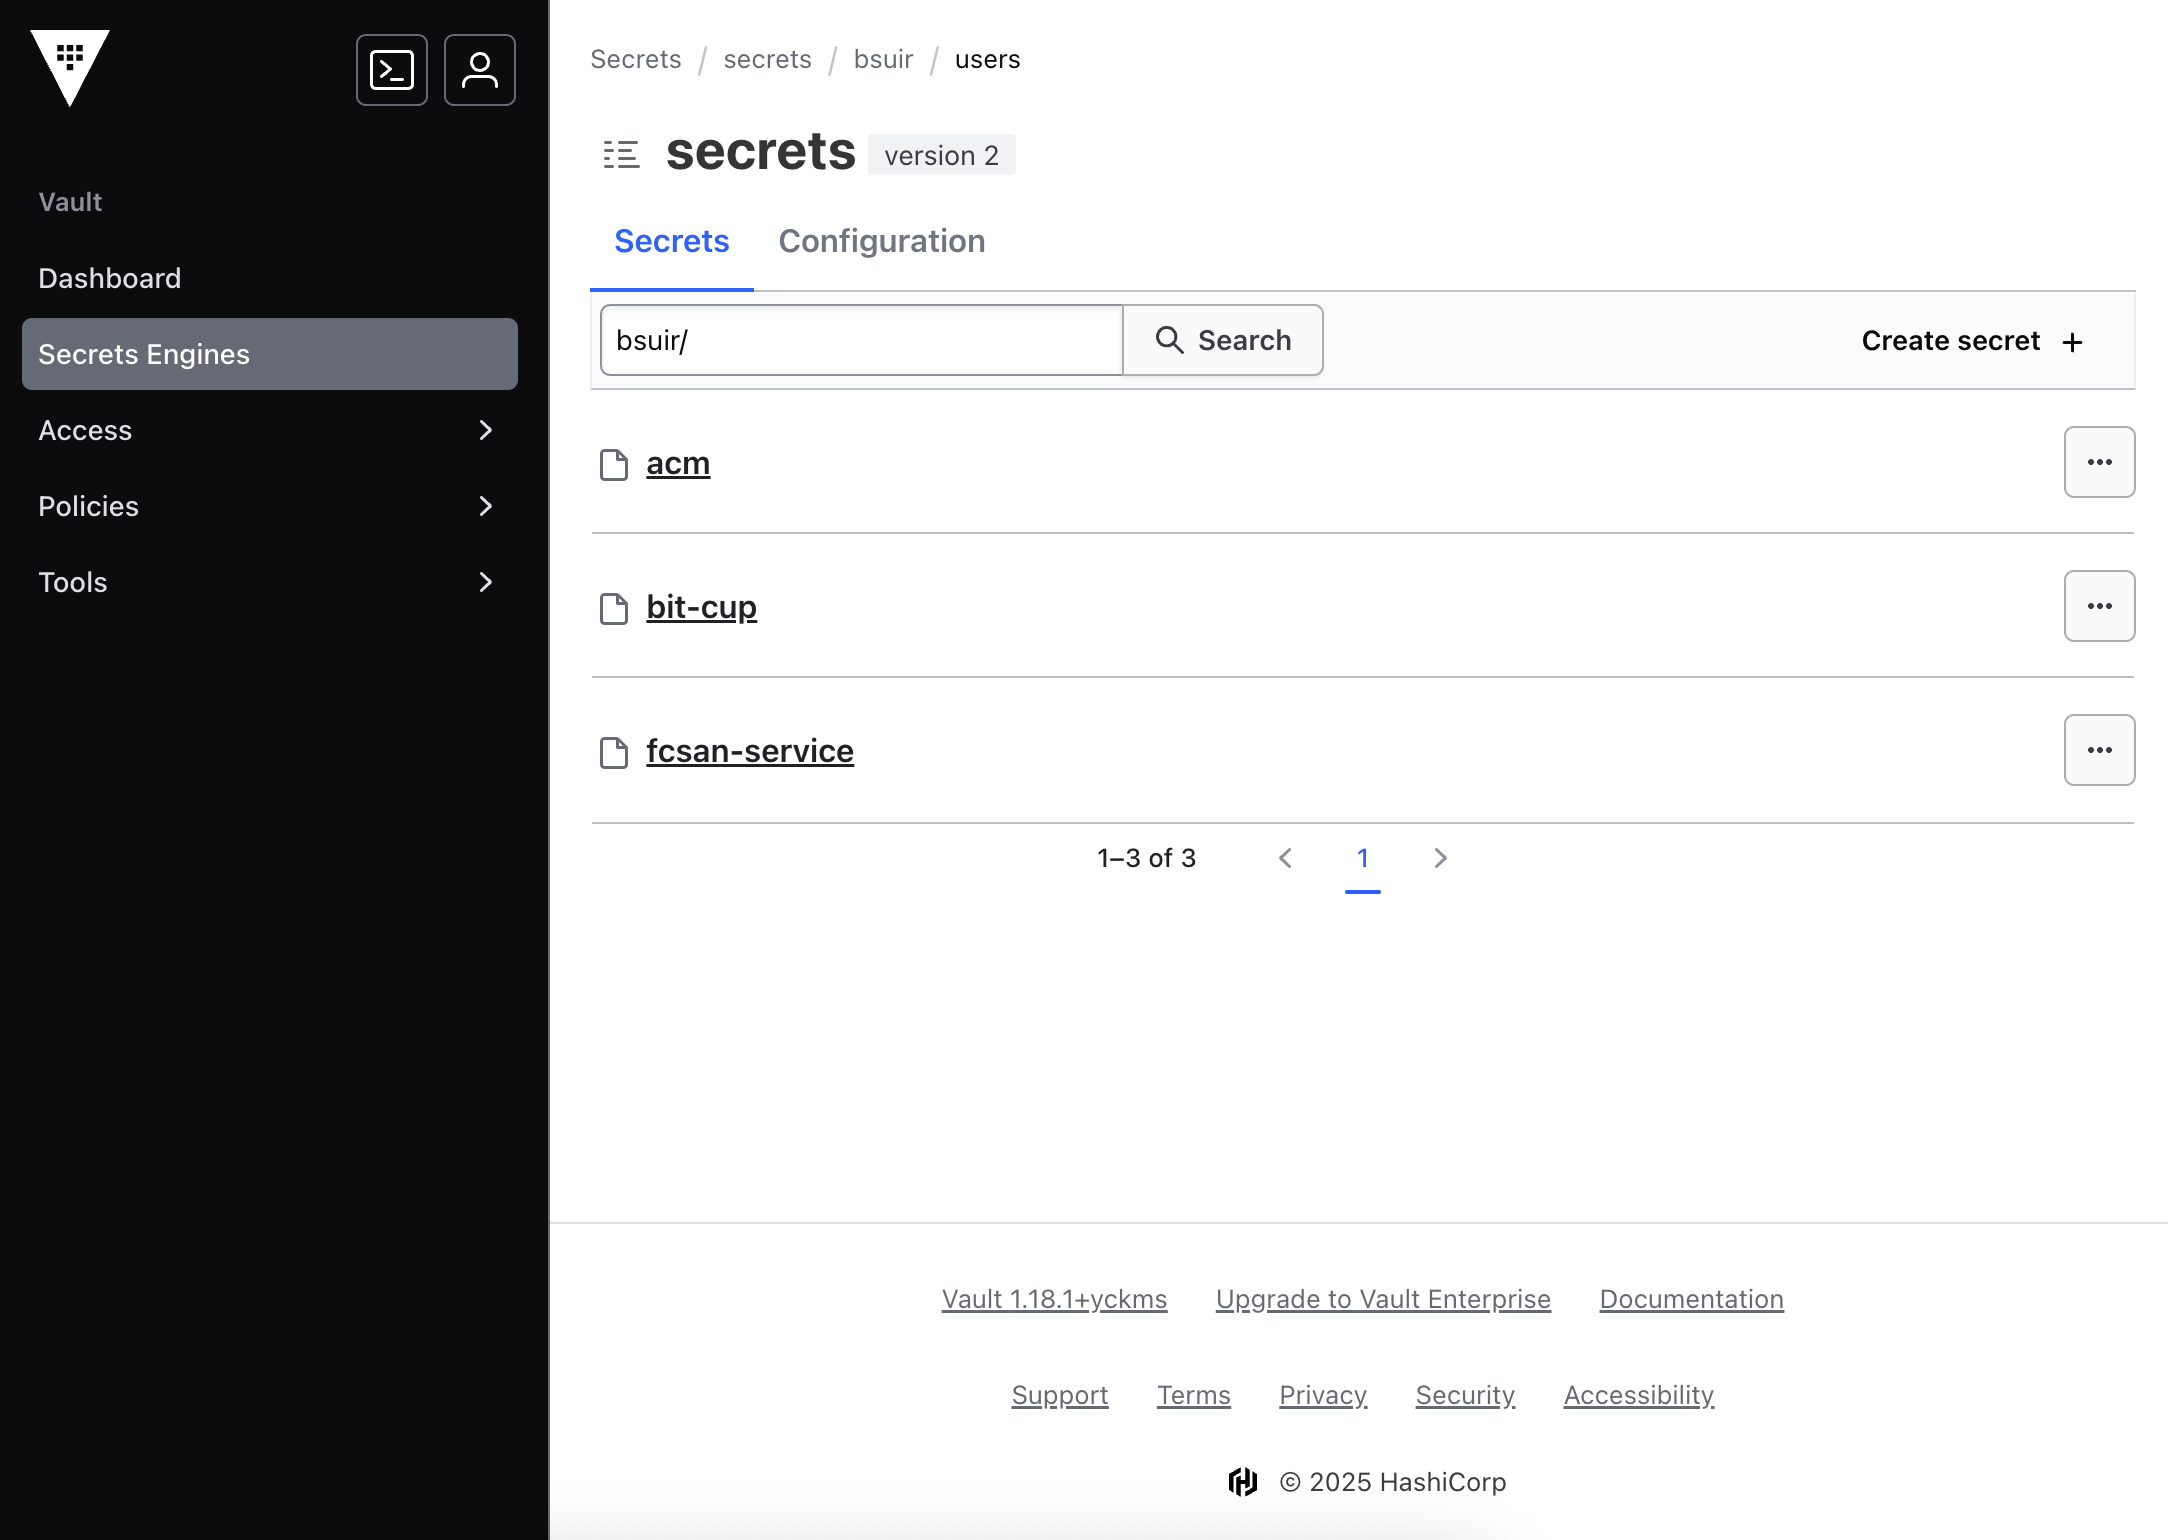
\includegraphics[width=0.7\linewidth]{\commonSecPathPrefix/../img/sec_6/vault_secrets.png}
    \caption{Обзор хранилищ секретов в \textit{Vault}}
    \label{fig:user_guide:vault_secrets}
\end{figure}

Рисунок \ref{fig:user_guide:vault_secrets} демонстрирует общий обзор различных хранилищ секретов, доступных через интерфейс \textit{Vault}. Пользователю предоставляется интуитивно понятный инструмент для навигации по иерархии путей и работы с множеством движков секретов.

Ниже приведены основные функциональные возможности интерфейса.

Первый блок возможностей касается работы с движками секретов. \textit{Vault} поддерживает несколько типов движков (секретных бекендов):

\begin{enumerate}
    \item \textit{KV (Key-Value)} —- классическое хранилище ключ-значение для любых типов данных.
    \item \textit{Transit} —- движок для шифрования и расшифровки данных без сохранения самих секретов.
    \item \textit{PKI (Public Key Infrastructure)} —- управление сертификатами и инфраструктурой открытых ключей.
\end{enumerate}

Далее интерфейс позволяет просматривать дерево путей, где хранятся секреты, а также выполнять операции создания, удаления и редактирования отдельных элементов.

Пользователь может создавать новые записи, редактировать существующие данные или удалять устаревшие секреты с сохранением истории изменений.

Для движка \textit{KV} доступна версияция, которая позволяет отслеживать изменения секретов с момента создания и при необходимости возвращаться к предыдущим версиям. Также возможно задание времени жизни (\textit{TTL}) для автоматического удаления или ротации секретов.

Управление доступом реализовано на основе политик. \textit{Vault} использует модель политик на базе \textit{ACL}, позволяя гибко настраивать права чтения, записи и управления для отдельных пользователей и сервисов.

В дополнение к описанным функциям, в нашей инфраструктуре активно используется модуль \textit{PKI}, который обеспечивает автоматизацию процессов выпуска и управления цифровыми сертификатами.

\begin{figure}[ht]
    \centering
    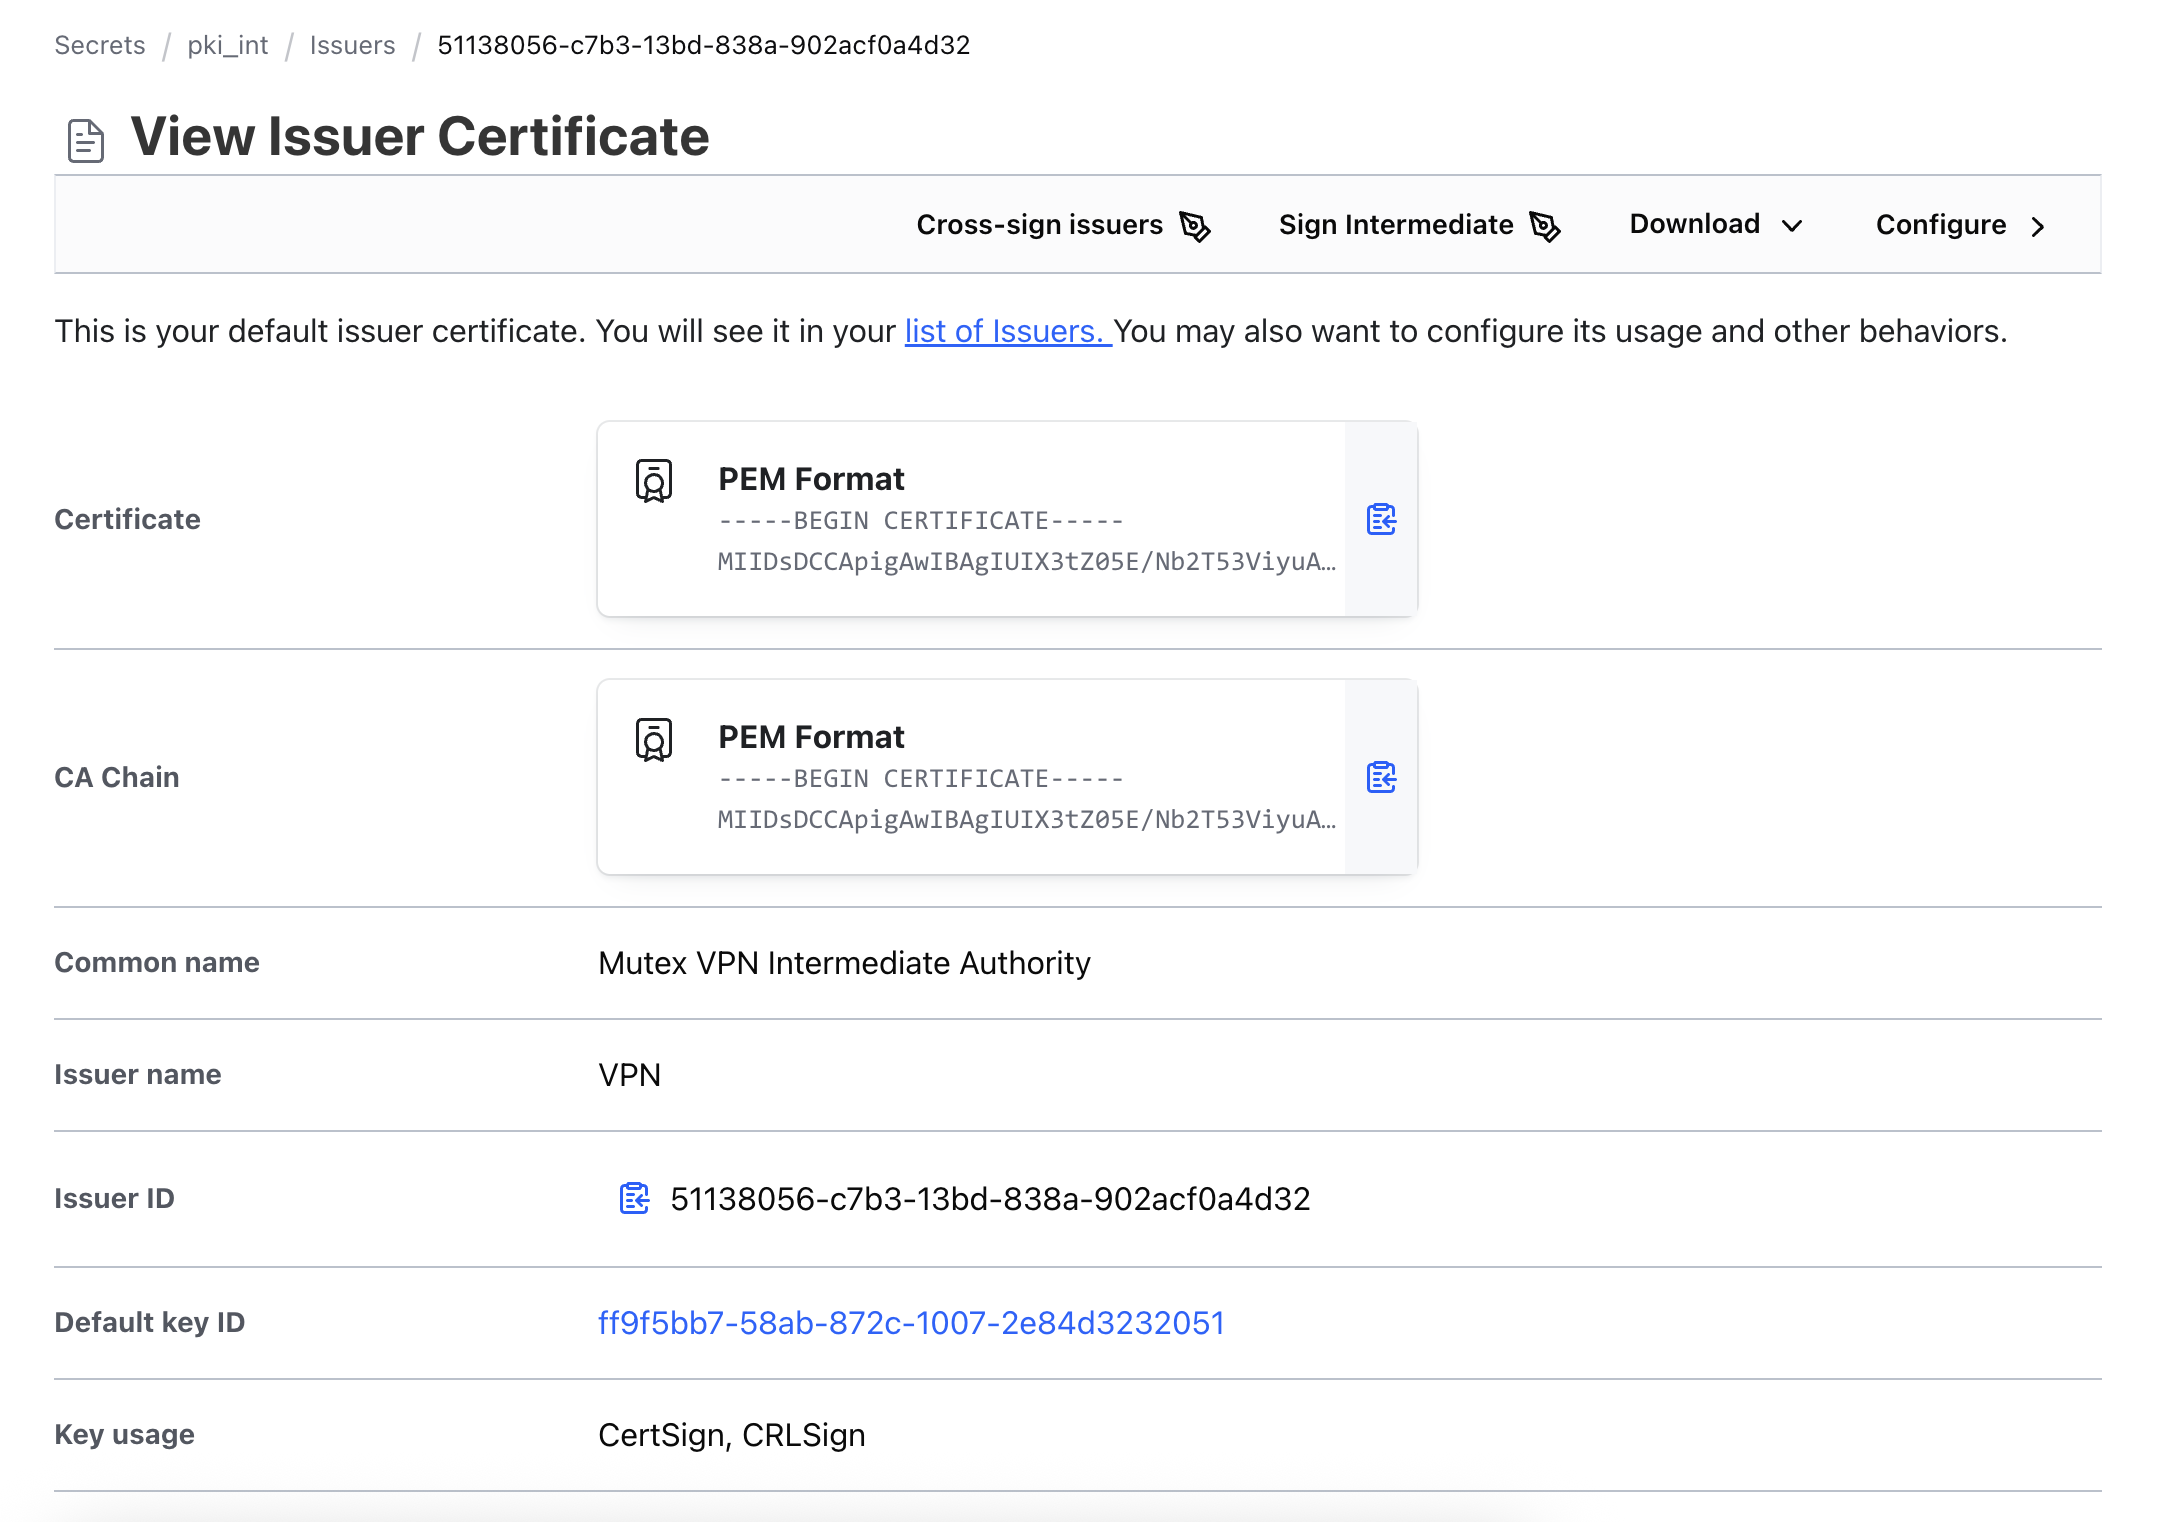
\includegraphics[width=0.7\linewidth]{\commonSecPathPrefix/../img/sec_6/vault_pki.png}
    \caption{Управление сертификатами и \textit{CA} в \textit{Vault PKI}}
    \label{fig:user_guide:vault_pki}
\end{figure}

На рисунке \ref{fig:user_guide:vault_pki} показан интерфейс управления сертификатами и центрами сертификации.

Модуль \textit{PKI} предоставляет следующие возможности:

\begin{enumerate}
    \item Выпуск и отзыв сертификатов. Автоматизированный процесс генерации сертификатов с возможностью их последующего отзыва при необходимости, что повышает безопасность коммуникаций.
    \item Настройка корневых и промежуточных центров сертификации (\textit{CA}). \textit{Vault} позволяет создавать и конфигурировать несколько уровней \textit{CA}, обеспечивая структурированное управление сертификатами и их цепочками доверия.
    \item Генерация списков отозванных сертификатов (\textit{CRL}). Поддерживается формирование актуальных списков отозванных сертификатов, необходимых для проверки подлинности.
\end{enumerate}

Кроме того, модуль \textit{PKI} позволяет:

\begin{enumerate}
    \item Управлять политиками выпуска сертификатов. Настраивать роли, ограничивающие параметры выдаваемых сертификатов (например, допустимые домены, время жизни, \textit{IP}-адреса).
    \item Проводить аудит операций. Вести подробный журнал всех действий с сертификатами и \textit{CA}, что позволяет контролировать безопасность и проводить расследования при необходимости.
\end{enumerate}

Стоит отметить, что интерфейс \textit{Vault} поддерживает интеграцию с системами единого входа (\textit{SSO}). Это упрощает управление правами доступа для сотрудников и сервисов в корпоративной инфраструктуре.

Благодаря перечисленным возможностям, \textit{HashiCorp Vault} является важной частью построения отказоустойчивой и безопасной \textit{IT}-инфраструктуры компании, обеспечивая комплексную защиту конфиденциальных данных и надежное управление ключами.

\subsection{Управление задачами и документацией в \textit{YouTrack}}

\textit{YouTrack}\cite{youtrack} применяется для управления задачами, спринтами и внутренними вики-документами. Поддерживается гибкая система фильтрации, визуальных представлений и экспорта данных.

\begin{figure}[ht]
    \centering
    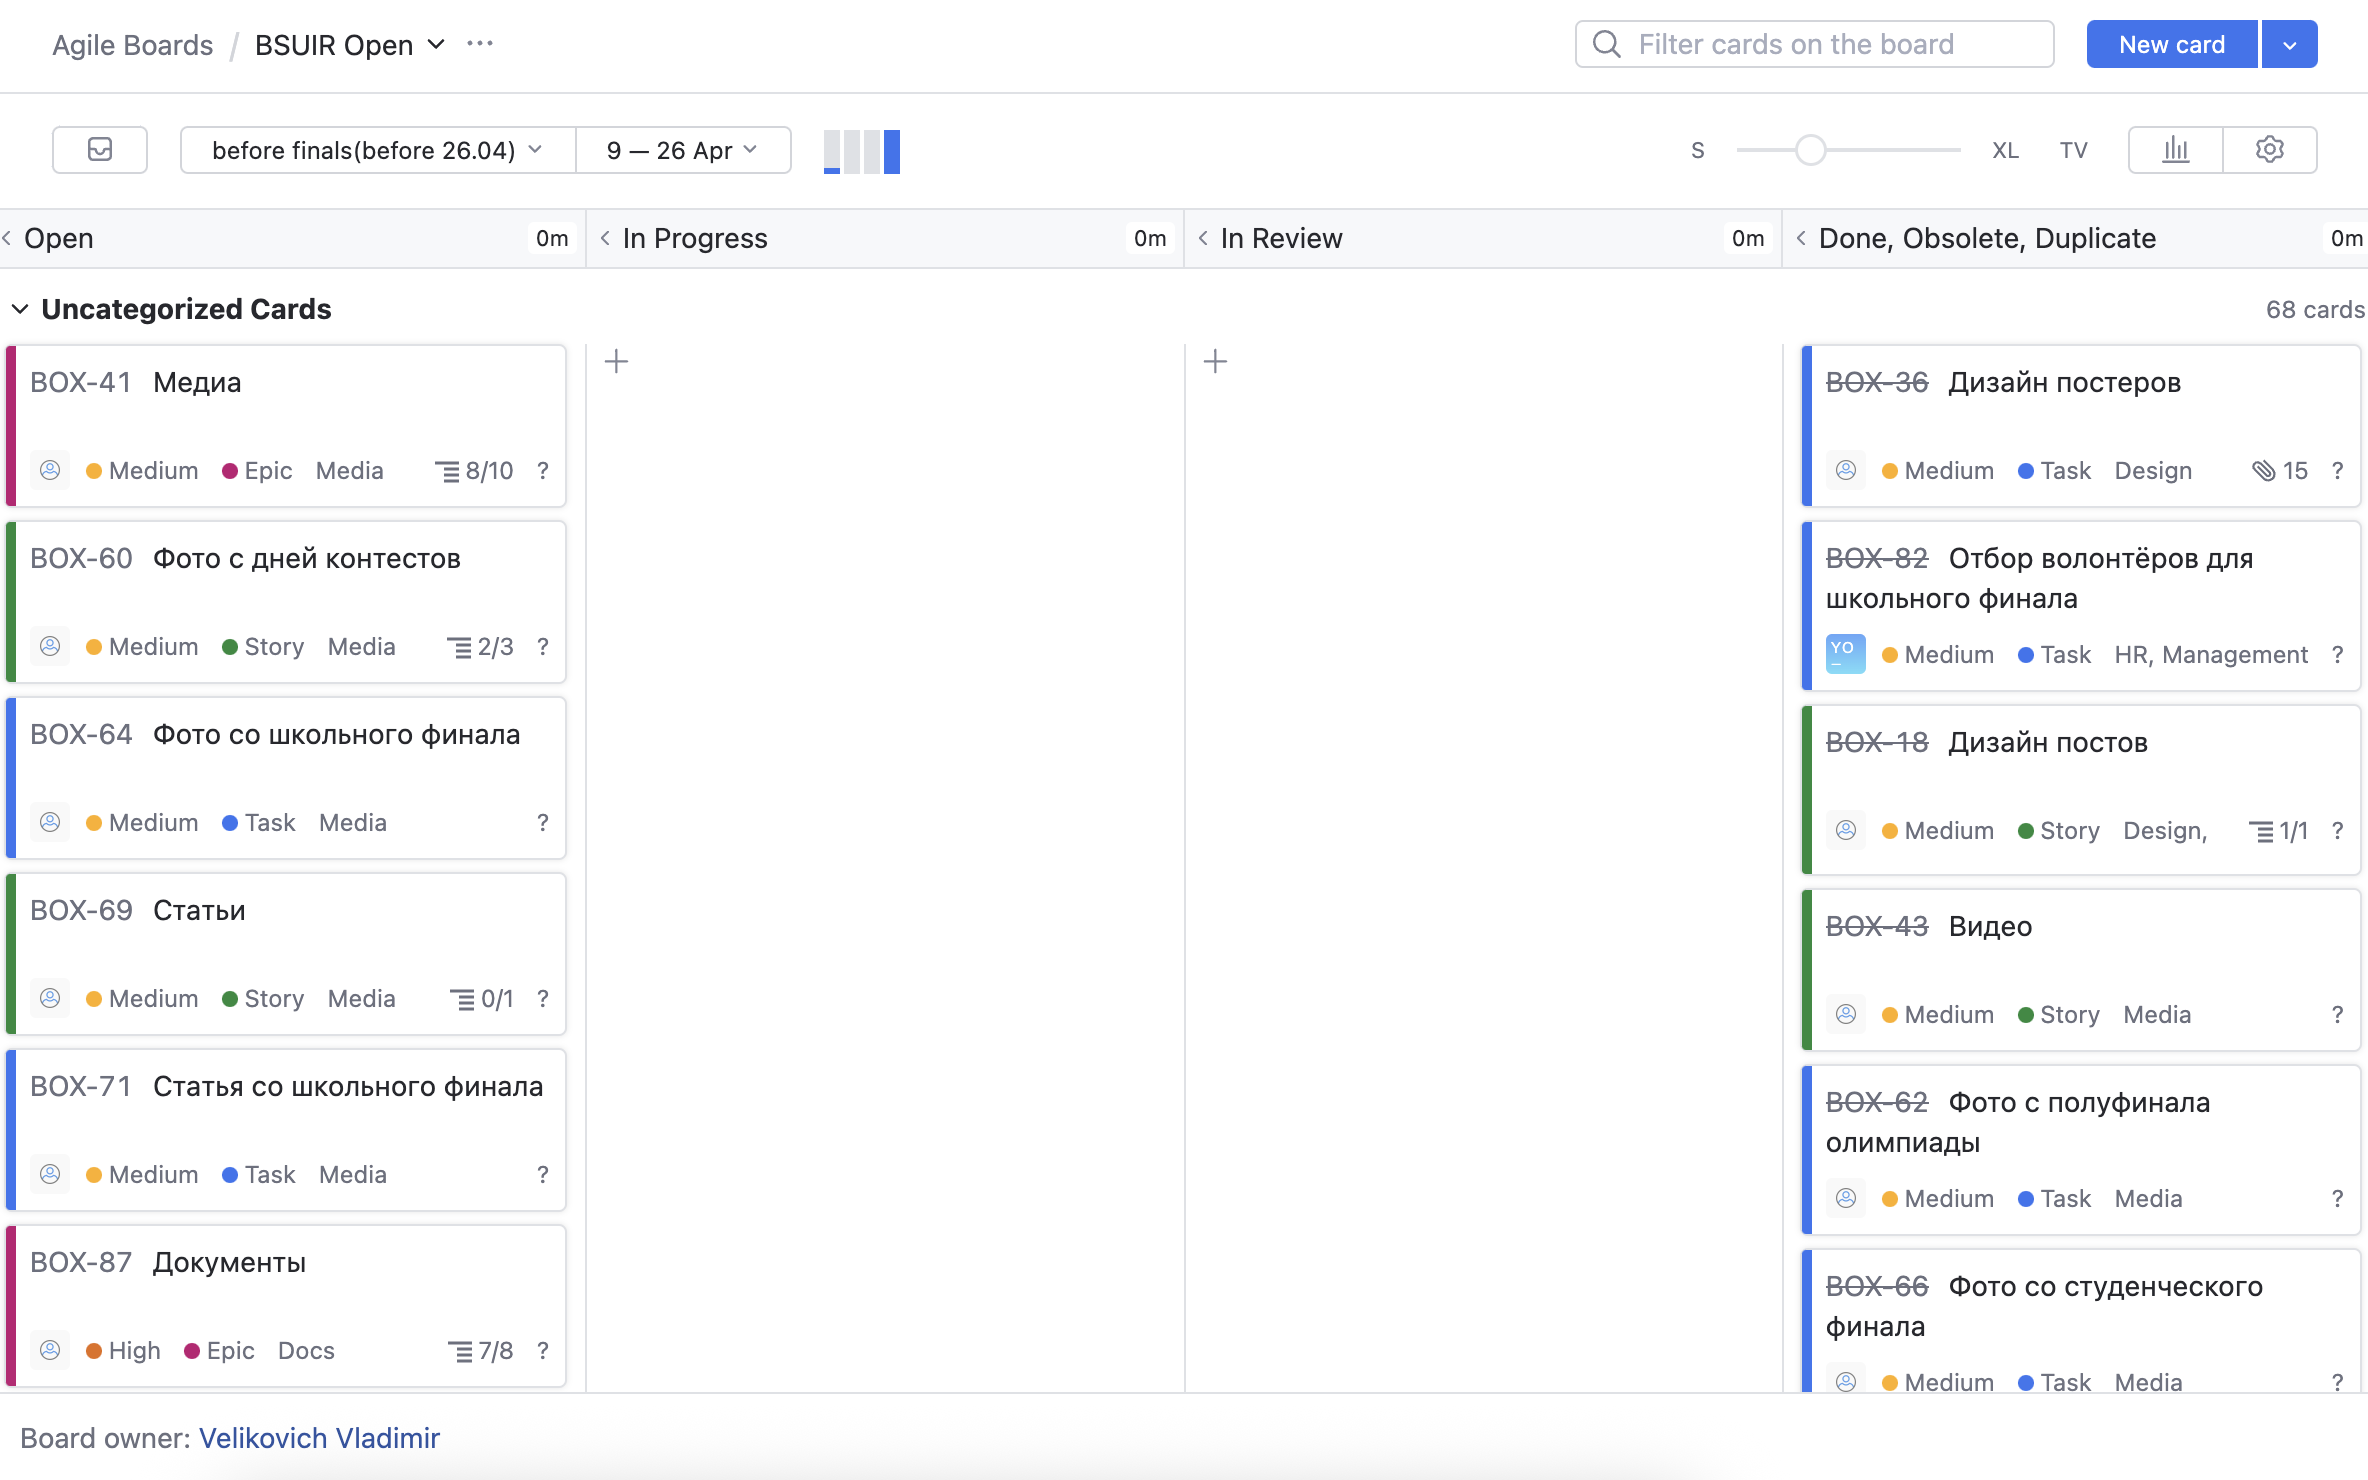
\includegraphics[width=0.7\linewidth]{\commonSecPathPrefix/../img/sec_6/yt_kanban.png}
    \caption{Доска задач в виде \textit{Kanban} в системе \textit{YouTrack}}
    \label{fig:user_guide:yt_kanban}
\end{figure}

\begin{itemize}
    \item колонки статусов: \textit{To Do}, \textit{In Progress}, \textit{Done};
    \item карточки с метками, приоритетом, исполнителем;
    \item фильтрация по тегам, проектам и пользователям;
    \item автоматическая синхронизация изменений.
\end{itemize}

Данный функционал позволяет удобно организовывать и контролировать процесс выполнения задач, обеспечивая прозрачность и упрощая взаимодействие между участниками команды. Пользователи могут быстро находить нужные задачи, отслеживать их статус и при необходимости корректировать распределение ресурсов для достижения поставленных целей.

\begin{figure}[ht]
    \centering
    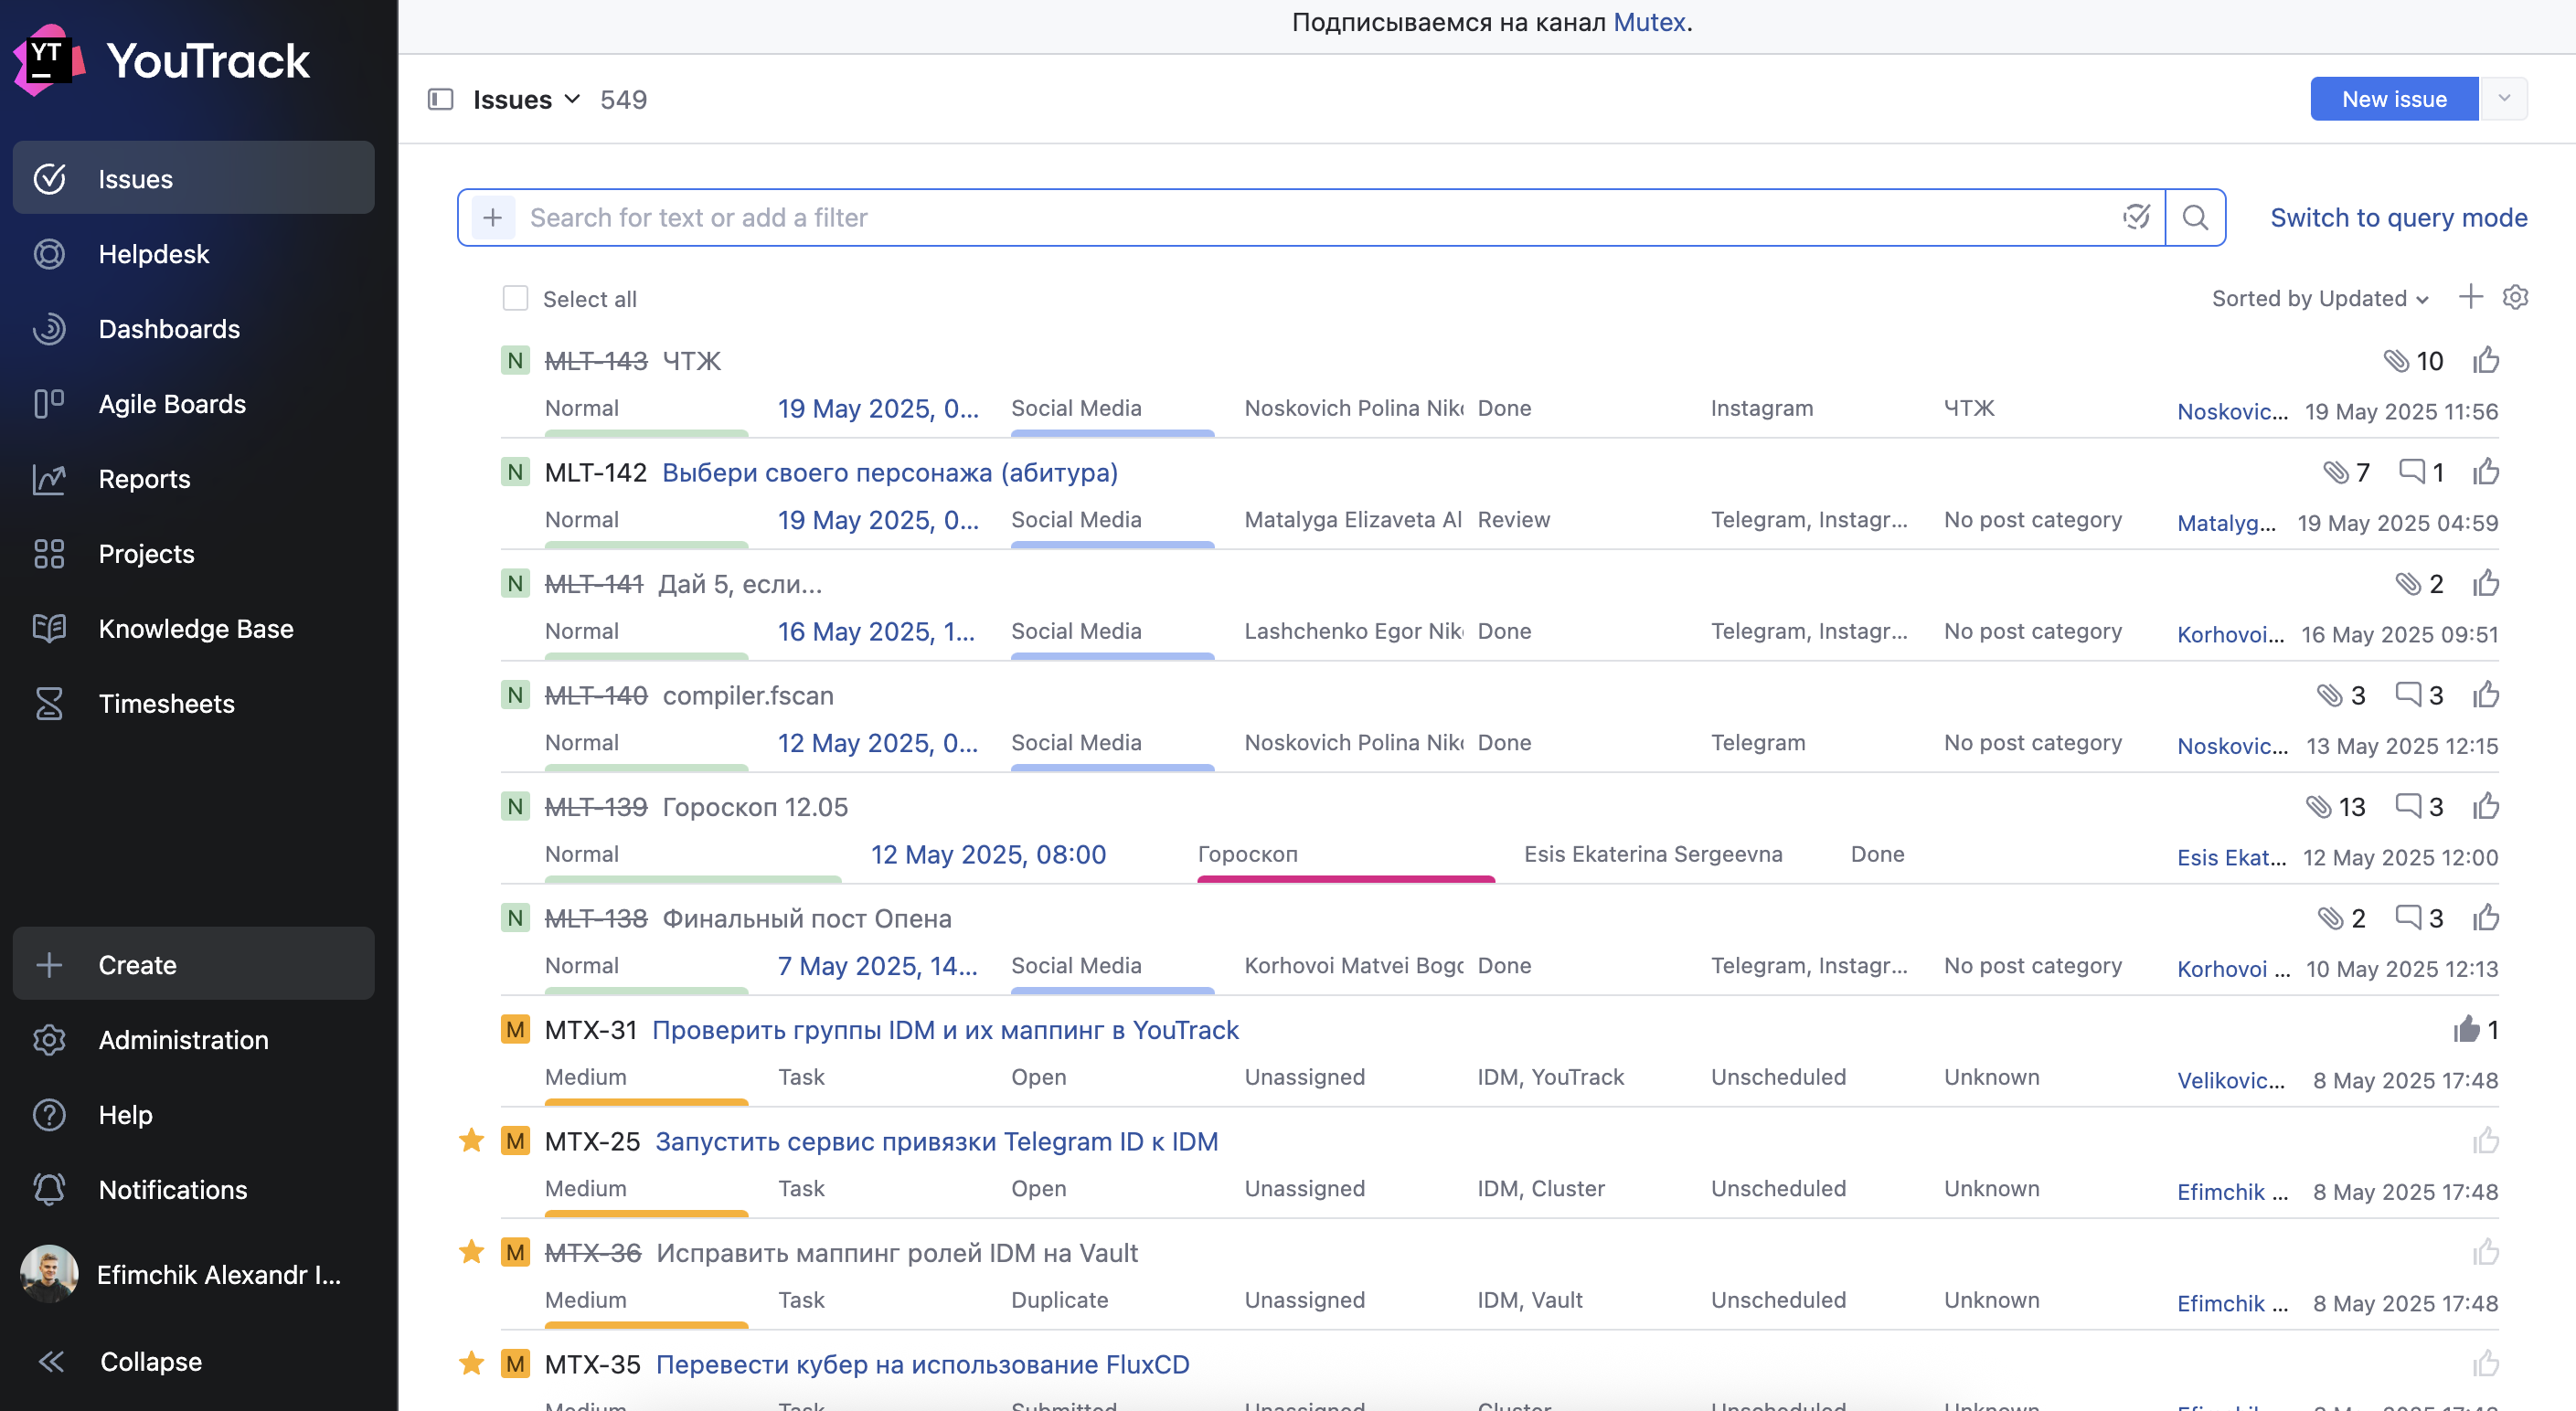
\includegraphics[width=0.7\linewidth]{\commonSecPathPrefix/../img/sec_6/yt_issues.png}
    \caption{Список задач в виде таблицы в системе \textit{YouTrack}}
    \label{fig:user_guide:yt_issues}
\end{figure}

Табличный вид списка задач в системе \textit{YouTrack} предоставляет пользователю удобный и наглядный инструмент для работы с большим объёмом задач. Интерфейс позволяет быстро находить, фильтровать и редактировать задачи, что значительно повышает эффективность управления проектами.

\begin{itemize}
    \item компактное отображение задач;
    \item язык фильтрации \textit{YQL};
    \item пакетное редактирование и экспорт.
\end{itemize}

\begin{figure}[ht]
    \centering
    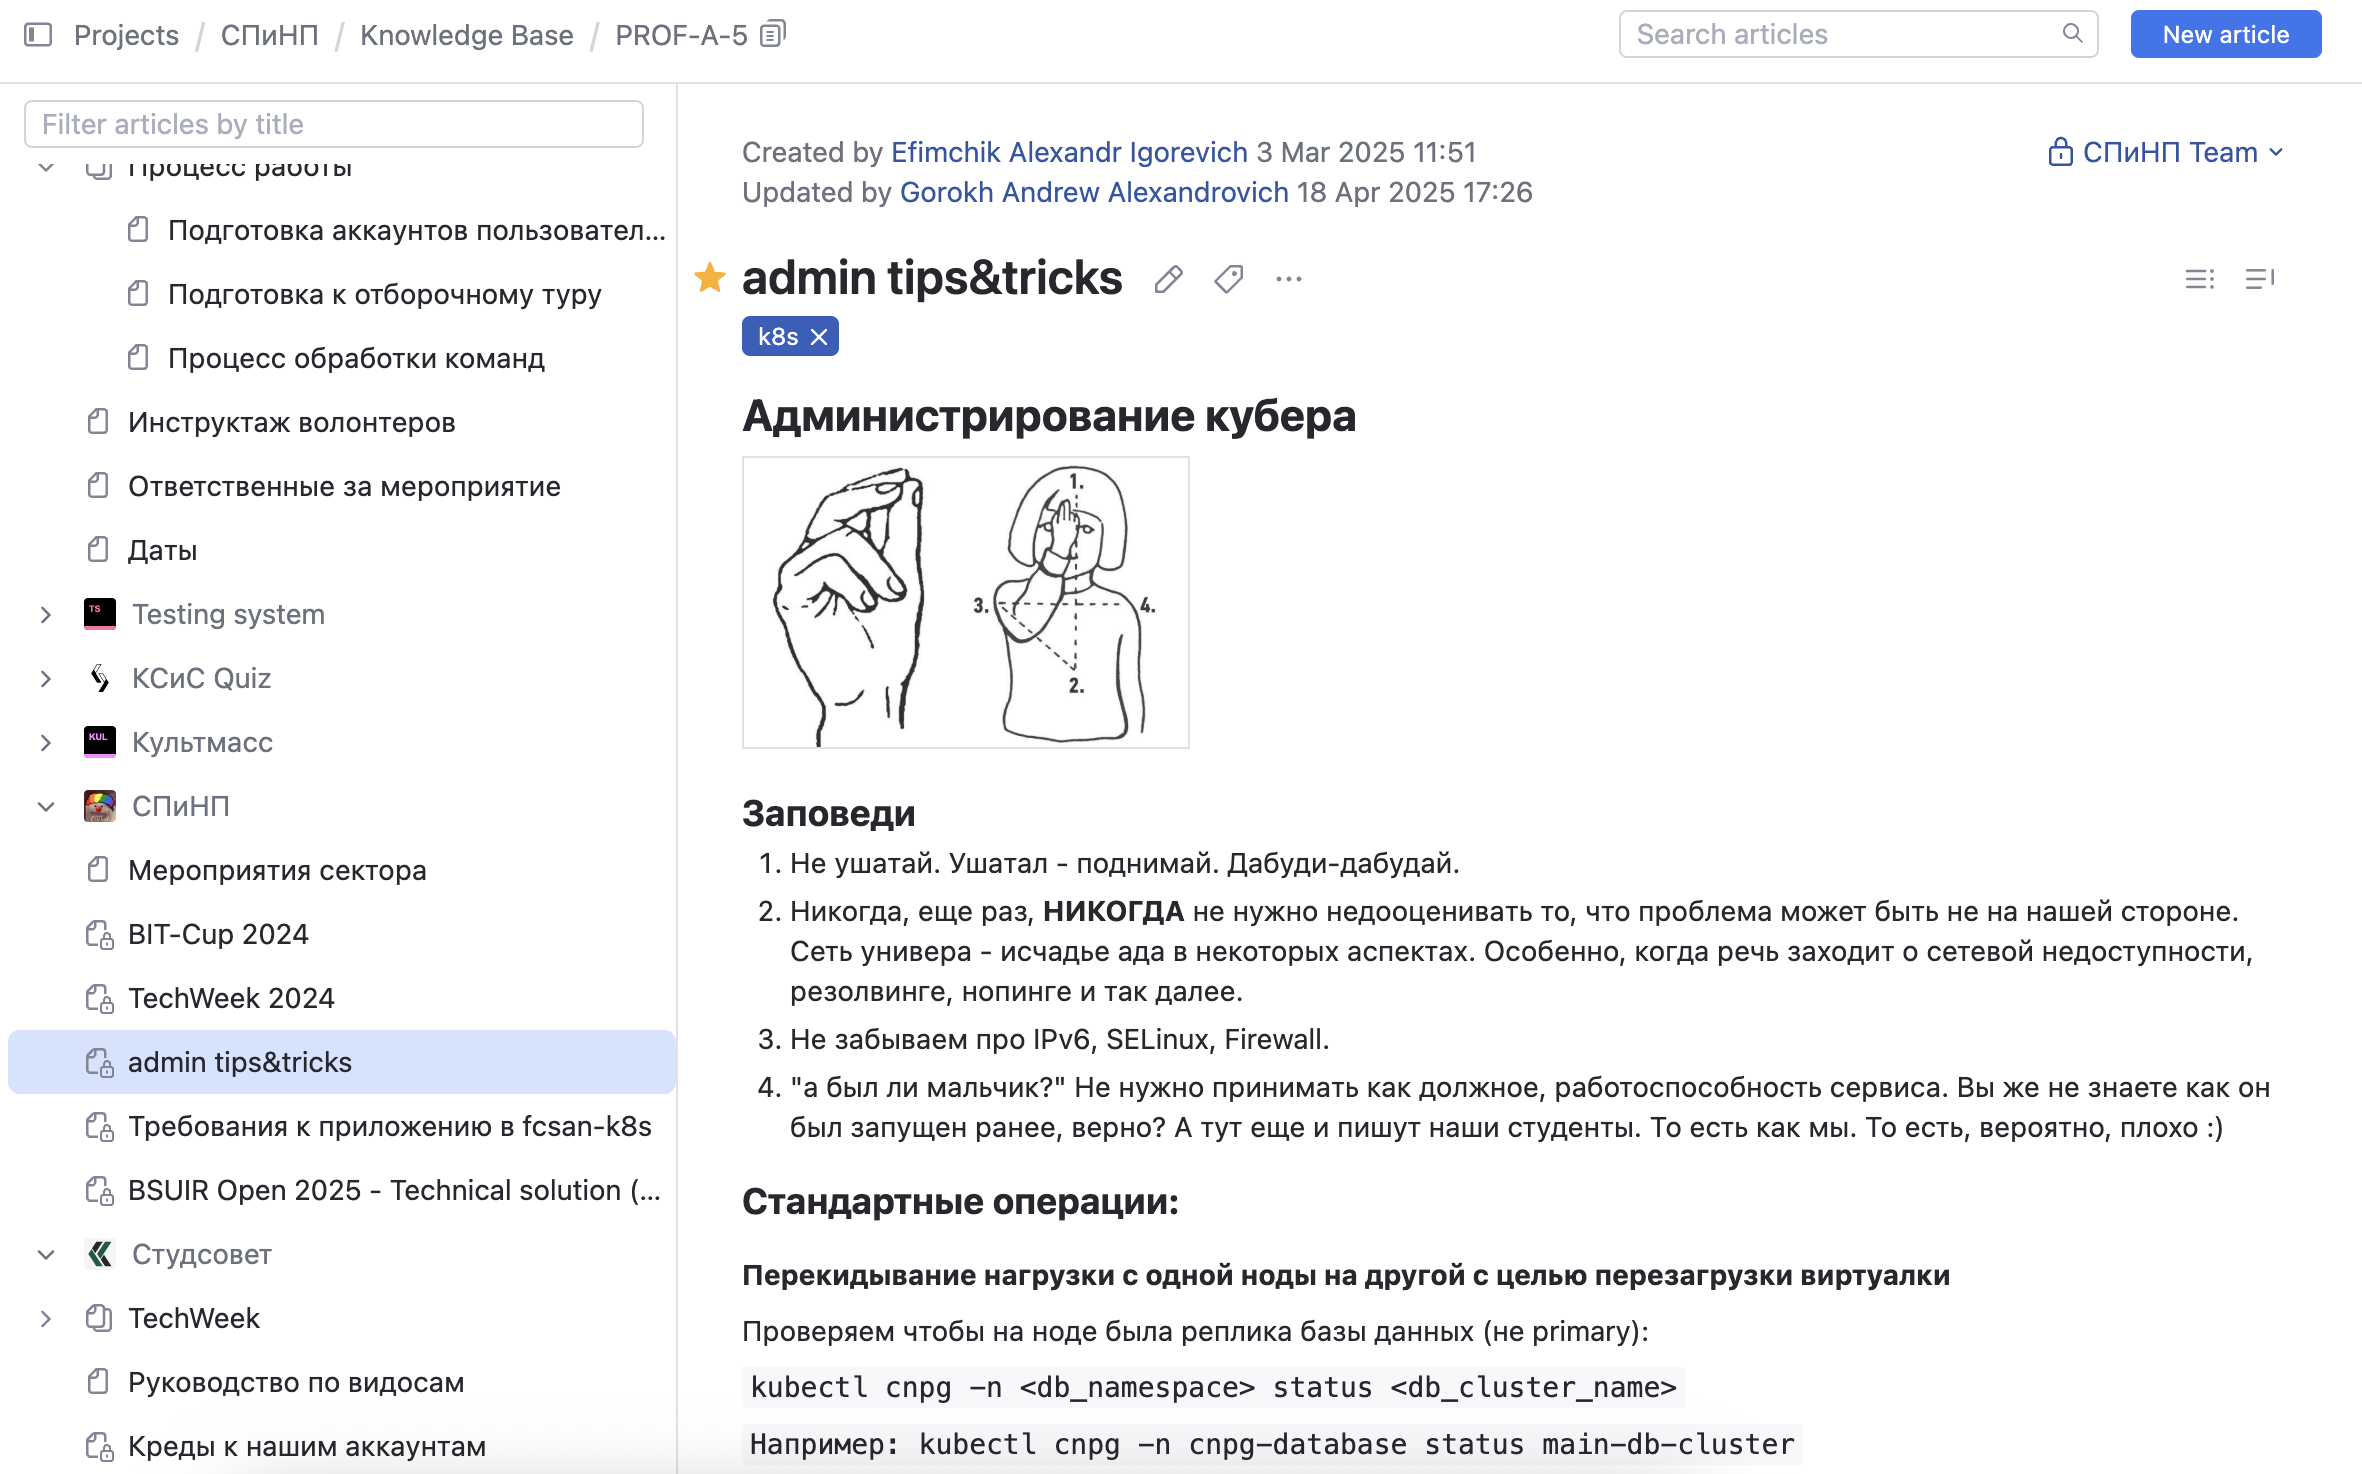
\includegraphics[width=0.7\linewidth]{\commonSecPathPrefix/../img/sec_6/yt_docs.png}
    \caption{Раздел документации в системе \textit{YouTrack}}
    \label{fig:user_guide:yt_docs}
\end{figure}

\begin{itemize}
    \item структура документации в виде дерева;
    \item поддержка \textit{Markdown};
    \item управление доступом на уровне страниц.
\end{itemize}

\subsection{Менеджер паролей \textit{Vaultwarden}}

Для безопасного хранения учетных записей и доступа к сервисам используется \textit{Vaultwarden}\cite{vaultwarden} -- облегчённая версия популярного менеджера \textit{Bitwarden}.

\begin{itemize}
    \item управление логинами, картами, записями и заметками;
    \item встроенный генератор паролей;
    \item двухфакторная аутентификация (\textit{TOTP});
    \item подключение к внешним провайдерам авторизации;
    \item поддержка папок, поиска, экспорта.
\end{itemize}

Приведённые возможности делают \textit{Vaultwarden} удобным инструментом для централизованного и безопасного хранения конфиденциальной информации. Интерфейс интуитивно понятен и адаптирован как для веб-версии, так и для мобильных клиентов.

\begin{figure}[ht]
    \centering
    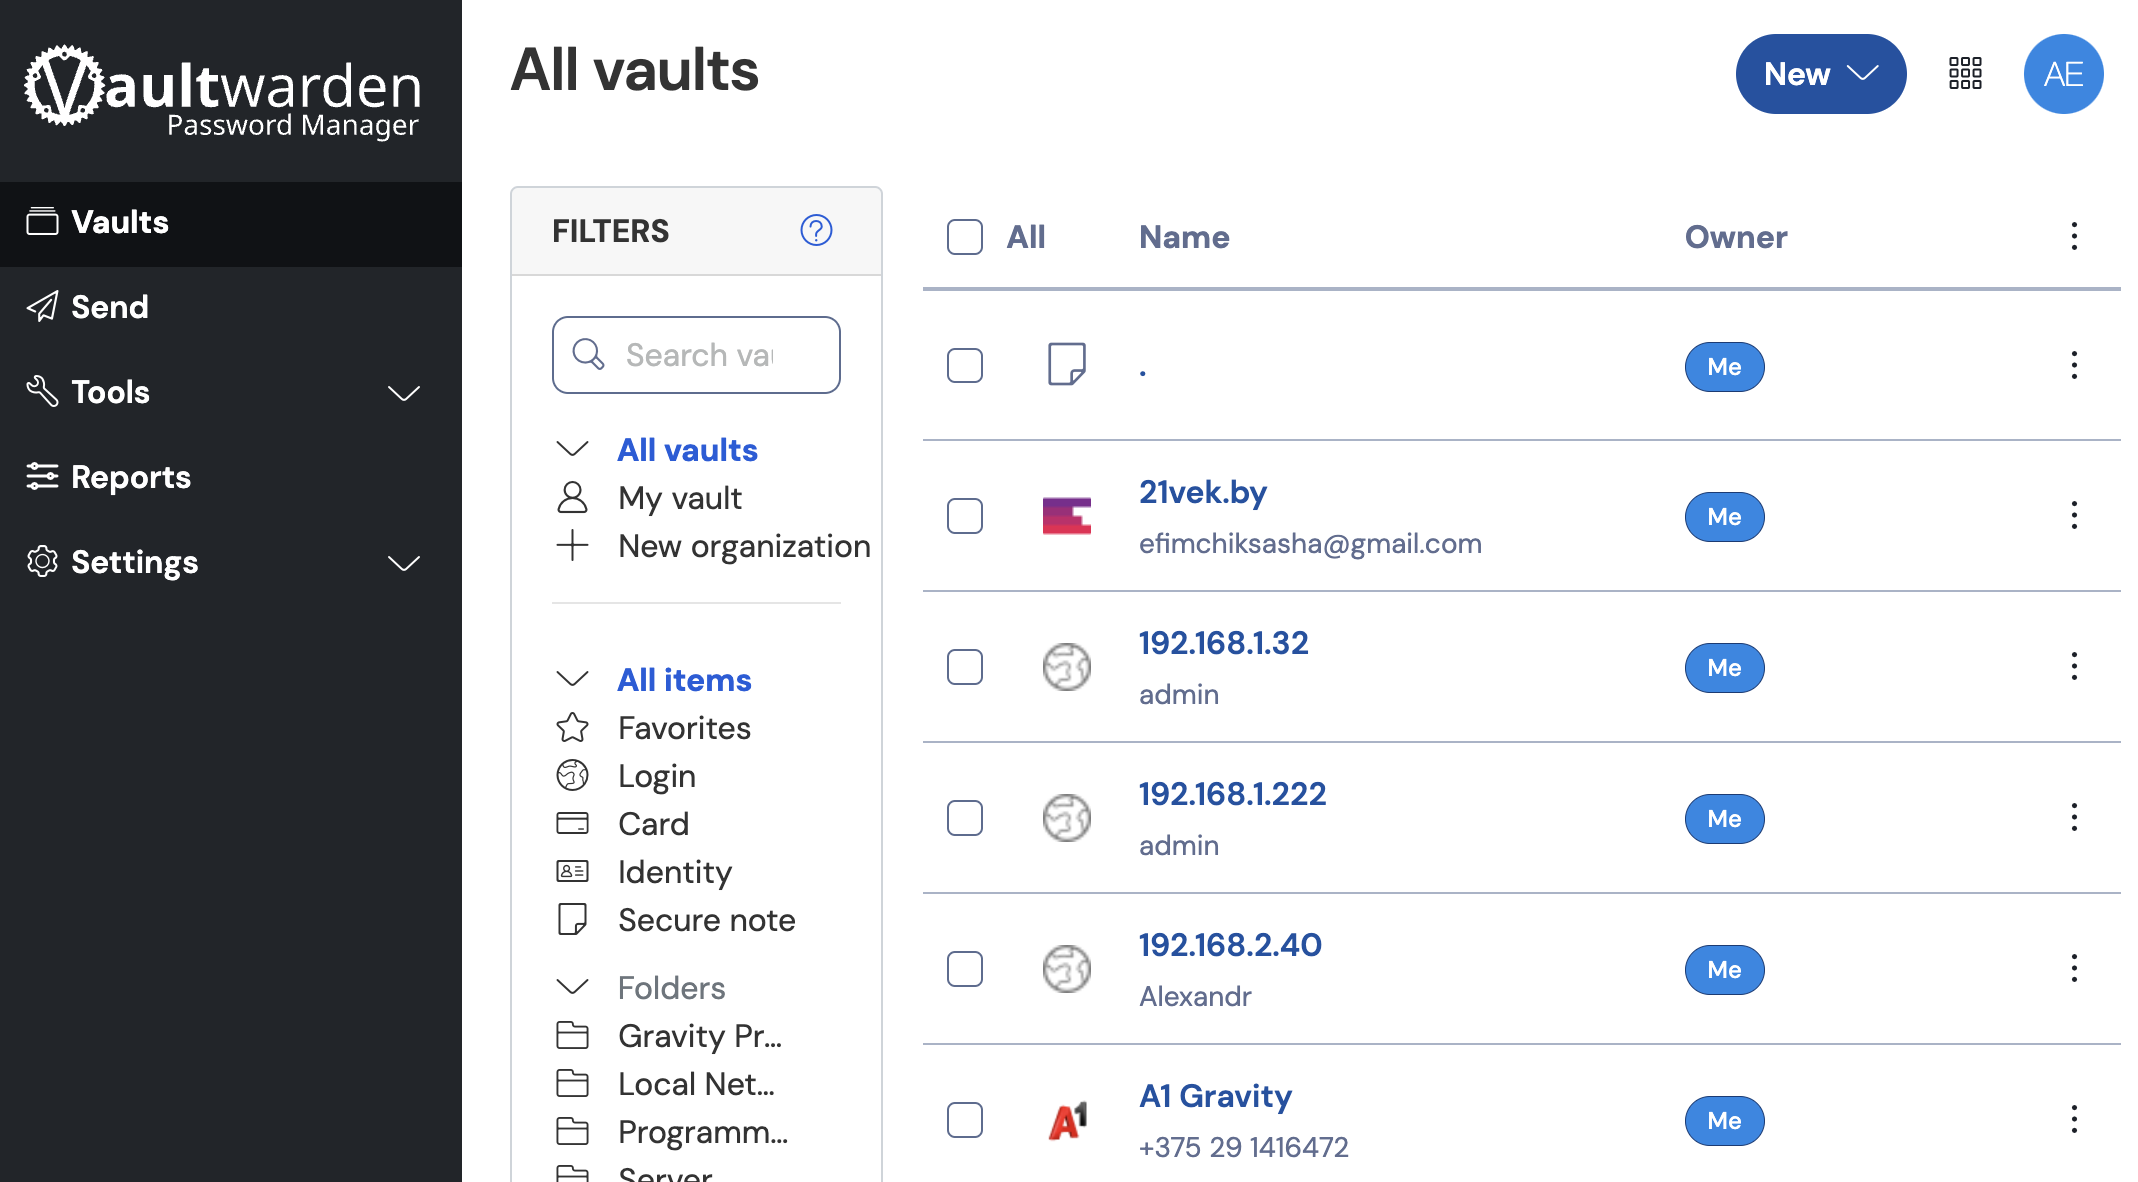
\includegraphics[width=0.6\linewidth]{\commonSecPathPrefix/../img/sec_6/vw.png}
    \caption{Интерфейс менеджера паролей \textit{Vaultwarden}}
    \label{fig:user_guide:vw}
\end{figure}

Вход в систему осуществляется по \textit{HTTPS}, данные хранятся в зашифрованном виде с использованием ключей, защищённых мастер-паролем пользователя.

Пользовательский интерфейс \textit{Vaultwarden} позволяет удобно и быстро управлять всеми сохранёнными учетными данными. Пользователи могут создавать новые записи, редактировать существующие и организовывать их по папкам для удобства навигации.

Также доступна функция автоматического заполнения форм и логинов в браузерах и мобильных приложениях, что значительно упрощает процесс аутентификации на различных сервисах и снижает риск использования слабых паролей.

Благодаря поддержке двухфакторной аутентификации, пользователи получают дополнительный уровень защиты своих данных. Возможность интеграции с внешними провайдерами авторизации позволяет использовать корпоративные учетные записи для доступа, что упрощает управление правами и повышает безопасность.

Кроме того, \textit{Vaultwarden} обеспечивает возможность экспорта и импорта данных, что облегчает миграцию с других менеджеров паролей и резервное копирование важной информации.
